\documentclass[review]{elsarticle}

\usepackage{amssymb,amsmath,amsthm,amsfonts}
%\usepackage[margin=1.0in]{geometry}
%\usepackage{fancyhdr} % required for custom header
%\usepackage{graphicx}
%\usepackage{listings}
%\usepackage{courier}
%\usepackage[usenames,dvipsnames]{color}
\usepackage[maxfloats=40]{morefloats}
%\usepackage{caption}
%\usepackage{subcaption}
%\usepackage{natbib}
%\usepackage{setspace}
%\doublespacing

%set up the header
%\pagestyle{fancy}
%\lhead{Trever Hines}
%\chead{El Mayor Postseismic}
%\rhead{\today}

%\setlength{\headheight}{15pt}
%\renewcommand\headrulewidth{1.0pt} % Size of the header rule

%% Title
%%------------------------------------------------------------------------------
\title{	
Rheologic constraints on the upper mantle from five years of postseismic deformation following the El Mayor-Cucapah earthquake}
\author{T. T. Hines\fnref{fn}}
\author{E. A. Hetland\fnref{fn}}
\fntext[fn]{Department of Earth and Environmental Sciences, University of Michigan, Ann Arbor, MI, USA}

\begin{document}
\begin{abstract}
Five years of postseismic deformation following the  Mw7.2 El Mayor-Cucapah earthquake reveals transient deformation that decays back to its preseismic trend after about 3 years at epicentral distances greater than $\sim200$ km. In the near-field, we observe rapid transience that decays to a sustained rate which exceeds its preseismic trend.  We attempt to determine the mechanisms driving this observed deformation, where we consider afterslip at seismogenic depths and viscoelastic relaxation in the lower crust and upper mantle as candidate mechanisms.  We find that early, rapid, near-field deformation can be explained with afterslip on the portion of the fault that ruptured coseismically, while the later, sustained, near-field deformation can be explained with either continued afterslip or a stead-state viscosity of $\sim10^{19}$ Pa s in the lower crust. The trend in far-field deformation is best explained with a transient viscosity of $\sim10^{18}$ Pa s in the upper mantle. We argue that a transient rheology in the mantle is preferable over a Maxwell rheology because it better predicts the observable postseismic deformation and also because it does not conflict with the generally higher, steady-state viscosities inferred from studies on geophysical processes occurring over longer time scales.
    
\end{abstract}
\maketitle

%%%%%%%%%%%%%%%%%%%%%%%%%%%%%%%%%%%%%%%%%%%%%%%%%%%%%%%%%%%%%%%%%%%%%%%%%%%%%%
%%%%%%%%%%%%%%%%%%%%%%%%%%%%%%%%%%%%%%%%%%%%%%%%%%%%%%%%%%%%%%%%%%%%%%%%%%%%%%
\section{Introduction}
Ground deformation in the years following a large ($\gtrsim$Mw7) earthquake provides insight into the mechanical behaviour of the crust and upper mantle. It has long been recognized that interpretations of postseismic deformation can be ambiguous because multiple postseismic deformation mechanisms can have qualitatively similar surface expressions \citep[e.g.][]{Savage1990}. Thanks to the dense geodetic network deployed throughout the 2000s as part of the Plate Boundary Observatory, the April 4, 2010, Mw7.2 El Mayor-Cucapah earthquake in Baja California produced observable postseismic deformation at more GPS stations than any other earthquake in California to date. With such a large collection of data, we attempt to discern the mechanisms driving postseismic deformation following the El Mayor-Cucapah earthquake, where we consider both afterslip and viscoelastic relaxation in the lower crust and upper mantle as candidate mechanisms. 

Previous studies which have modelled postseismic deformation following the El Mayor-Cucapah earthquake include \citet{Pollitz2012}, \citet{Gonzalez-ortega2014}, \citet{Spinler2015}, and \citet{Rollins2015}. Of these studies, \citet{Gonzalez-ortega2014} and \citet{Rollins2015} have attempted to describe the postseismic deformation with afterslip in an elastic half-space.  \citet{Gonzalez-ortega2014} described five months of postseismic deformation, observed by near-field ($\lesssim$ 50 km from the rupture) campaign GPS and InSAR, with afterslip and contraction on the coseismically ruptured fault. \citet{Gonzalez-ortega2014} noted that their preferred model underestimated the GPS displacements for stations $\gtrsim 25$ km from the rupture and suggested that it could be the result of unmodelled viscoelastic relaxation.  Using continuous GPS stations, which are mostly north of rupture zone, \citet{Rollins2015} found that three years of postseismic deformation can be adequately explained by afterslip, albeit with an implausibly large amount of slip inferred on the least constrained, southern-most fault segment. Here, we suggest the afterslip inferred by \citet{Rollins2015} may have been acting as a proxy for distributed relaxation in the upper mantle. 

\citet{Pollitz2012}, \citet{Rollins2015} and \citet{Spinler2015} have explored viscoelastic relaxation in the lower crust and upper mantle as a potential postseismic deformation mechanism. The rheology of the crust and mantle is largely unknown and so modelling postseismic deformation with viscoelastic relaxation requires one to assume a rheologic model and then find the best fitting rheologic parameters.  The inference of these rheologic parameters is a computationally expensive non-linear inverse problem which is typically approached with a forward modelling grid search method.  Consequently, a simplified structure for the lithosphere must be made to minimize the number of rheologic parameters that need to be estimated.  For example, it is commonly assumed that the lithosphere consists of only three homogeneous, Maxwell viscoelastic layers, which may be an inadequate representation of the lithosphere \citep{Riva2009,Hines2013}. To further reduce the model space dimensions being search, it is also necessary to make simplifying assumptions about the nature of afterslip. For example, one can assume a frictional model for afterslip and parametrize afterslip in terms of the unknown rheologic properties of the fault \citep[e.g.][]{Johnson2009,Johnson2004}. One can also assume that afterslip does not persist for more than a few months and then model the later postseismic deformation assuming it to be the result of only viscoelastic relaxation \citep[e.g.][]{Pollitz2012,Spinler2015}. However, postseismic afterslip in similar tectonic settings has been observed to persist for decades following earthquakes \citep{Cakir2012,Cetin2014}. Neglecting to allow for sustained afterslip as a postseismic mechanism could then lead to a biased inference of lithospheric viscosity. Indeed, the preferred viscoelastic model from \citet{Pollitz2012} significantly underestimates near-field deformation, which could be indicative of unmodelled continued afterslip.

In this study, we assume that both afterslip and viscoelastic relaxation can contribute to postseismic deformation. Modelling both of these mechanisms creates a high dimensional model space that must be searched with non-linear optimization methods. We first develop an initial postseismic model using the method described in \citet{Hines2015}. This method simultaneously estimate the afterslip and effective lithospheric viscosity structure necessary to describe the first 0.8 years of postseismic deformation following the El Mayor-Cucapah earthquake.  We then use the inferred effective viscosity structure to create a suite of postseismic models which are tested against the available 5 years of postseismic data.  Of the suite of models tested, we find that postseismic deformation following the El Mayor-Cucapah earthquake can be explained with afterslip beneath the Sierra Cucapah, a Zener rheology upper mantle with a transient viscosity that decays from $5\times10^{18}$ Pa s to $1\times10^{18}$ Pa s at 120 km depth, and a relatively stronger lower crust. 

\begin{figure}
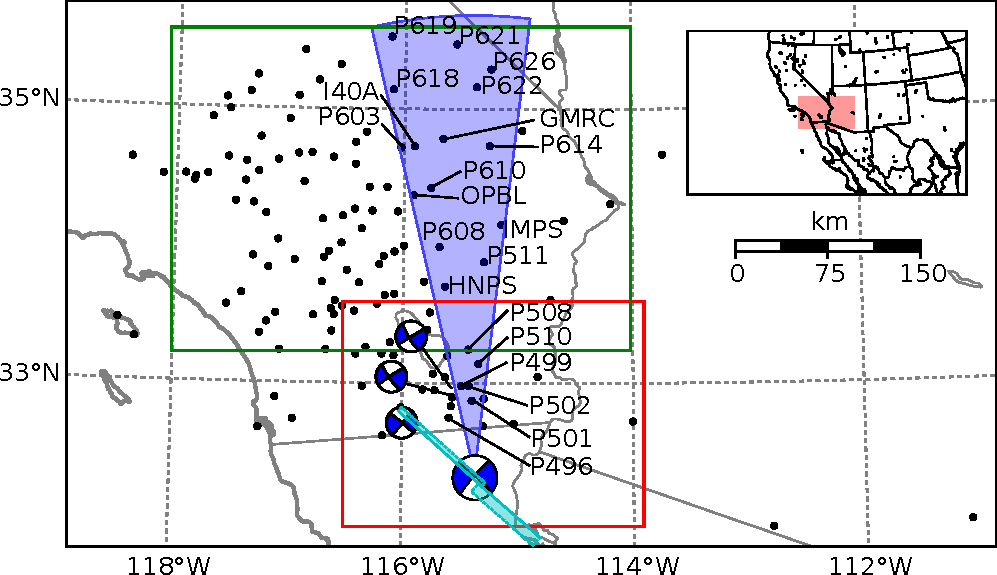
\includegraphics[scale=0.7]{Figures/ContextMap} 
\caption{Map of the region considered in this study.  The large focal mechanism is for the El Mayor-Cucapah earthquake and the three small focal mechanisms are for the Ocotillo earthquake and the two main shocks during the Brawley swarm.  The black dots indicate the locations of GPS stations used in this study.  The fault geometry used in this study is shown in cyan where dashed lines indicate buried edges of the fault segments.  The green and red boxes demarcate the extent of the near-field and far-field maps (figures \ref{fig:NearField} and \ref{fig:FarField}).  Stations within the blue sector, which highlights the area within 10$^\circ$ of the El Mayor-Cucapah P axis, are used in the record sections in Figures \ref{fig:RecordSectionElastic}, \ref{fig:RecordSection1}, and \ref{fig:RecordSection2}}.       
\label{fig:ContextMap}
\end{figure}

%%%%%%%%%%%%%%%%%%%%%%%%%%%%%%%%%%%%%%%%%%%%%%%%%%%%%%%%%%%%%%%%%%%%%%%%%%%%%%
%%%%%%%%%%%%%%%%%%%%%%%%%%%%%%%%%%%%%%%%%%%%%%%%%%%%%%%%%%%%%%%%%%%%%%%%%%%%%%
\section{Data Processing}\label{sec:Data}

We use continuous GPS position time series provided by University Navstar Consortium (UNAVCO) for stations within a 400 km radius about the El Mayor-Cucapah epicentre. We collectively describe the coseismic and postseismic displacements resulting from the El Mayor-Cucapah earthquake as $u_\mathrm{post}(t)$.  We consider the GPS position time series, $u_\mathrm{obs}(t)$, to be the superposition of $u_\mathrm{post}(t)$, secular tectonic deformation, annual and semi-annual oscillations, and coseismic offsets from significant earthquakes over the time span of this study.  The June 14, 2010, Mw5.8 Ocotillo earthquake and the Brawley swarm, which included an Mw5.5 and an Mw5.3 event on August 26, 2012, (Figure \ref{fig:ContextMap}) are the only earthquakes that produced noticeable displacements in any of the time series.  We treat the displacements resulting from the Brawley swarm as a single event because the time series are provided by UNAVCO as daily solutions. Although the Ocotillo earthquake had its own series of aftershocks \citep{Hauksson2011}, neither the Ocotillo earthquake nor the Brawley swarm produced detectable postseismic deformation and we model displacements resulting from these events with a Heaviside function, $H(t)$.  We then model $u_\mathrm{obs}(t)$ as 
\begin{equation}
  u_\mathrm{obs}(t) = u_\mathrm{pred}(t) + \epsilon
\end{equation}
where
\begin{equation}\label{TimeSeriesModel}
  \begin{split}  
    u_\mathrm{pred}(t) = &u_\mathrm{post}(t)H(t-t_\mathrm{emc}) + c_0 + c_1t + \\
                         &c_2\sin(2\pi t) + c_3\cos(2\pi t) + c_4\sin(4\pi t) + c_5\cos(4\pi t) + \\
                         &c_6H(t-t_\mathrm{oc}) + c_7H(t-t_\mathrm{bs}).
  \end{split}
\end{equation}
In the above equations, $t_\mathrm{emc}$, $t_\mathrm{oc}$ and $t_\mathrm{bs}$ are the times of the El Mayor-Cucapah earthquake, Ocotillo earthquake, and the Brawley swarm, respectively, $c_0$ through $c_7$ are unknown coefficients, and $\epsilon$ is the observation noise. We only estimate jumps associated with the Ocotillo earthquake and Brawley swarm for stations within 40 km of their epicentres. 

Stations which recorded displacements that clearly cannot be described by the aforementioned processes are not included in our analysis. This includes stations in the Los Angeles basin, where anthropogenic deformation can be larger than the postseismic signal that we are trying to estimate \citep{Bawden2001,Argus2005} . In order to ensure an accurate estimation of the secular deformation, we only use stations that were installed at least six months prior to El Mayor-Cucapah earthquake. Several GPS stations were installed after the El Mayor-Cucapah earthquake to improve the spatial resolution of postseismic deformation \citep{Spinler2015} and it is possible to subtract secular velocities derived from elastic block models \citep[e.g.][]{Meade2005} from velocities recorded at the newly installed stations to get an estimate of postseismic velocities. However, we use coseismic and postseismic displacements, rather than velocities, in our inverse method described in Section \ref{sec:Model}. We use displacements because estimating velocities from an already noisy displacement time series can introduce significant aleatoric and epistemic uncertainties depending on exactly how the estimation is done. This modelling choice prevents us from using the newly installed stations in Baja California for our analysis.   

The October 16, 1999, Mw7.1 Hector Mine earthquake, which occurred about 270 km north of the El Mayor-Cucapah epicentre, produced transient postseismic deformation which we do not wish to model, either mechanically or through empirical line fitting.  We thus restrict our analysis to deformation observed six years after the Hector Mine earthquake, which is when postseismic velocities at sites proximal to the Hector Mine epicentre are approximately constant \citep{Savage2009}. When appraising our model fit in Section \ref{sec:Model}, we see some systematic residuals in the vicinity of the Hector Mine epicentre, which may be the result of errors in the assumption that the trend in Hector Mine postseismic deformation is linear after six years.   

Studies of postseismic deformation typically assume a parametric form for $u_\mathrm{post}(t)$, such as one with a logarithmic or exponential time dependence \citep[e.g.][]{Savage2005a}.  However, by assuming a logarithmic or exponential form of $u_\mathrm{post}(t)$ we run the risk of over fitting the GPS time series and inferring a non-existent postseismic signal. We therefore do not assume any parametric form for $u_\mathrm{post}(t)$ and rather treat it as integrated Brownian motion, so that 
\begin{equation}
    \dot{u}_\mathrm{post}(t) = \sigma^2\int_0^t w(s) ds,
\end{equation}    
where $w(t)$ is white noise and the variance of $\dot{u}_\mathrm{post}(t)$ increases linearly with time by a factor of $\sigma^2$. We use a Kalman filtering approach to estimate $u_\mathrm{post}(t)$ and the unknown parameters in eq. (\ref{TimeSeriesModel}).  In the context of Kalman filtering, our time varying state vector is
\begin{equation}
    \mathbf{X}(t) = [u_\mathrm{post}(t),\dot u_\mathrm{post}(t), c_0, ..., c_7]
\end{equation}
and eq. (\ref{TimeSeriesModel}) is the observation function which maps the state vector to the GPS observations. We initiate the Kalman filter by assuming a prior estimate of $\mathbf{X}(t)$ at the first time epoch, denoted $\mathbf{X}_{1|0}$, which has a sufficiently large covariance, denoted $\mathbf{\Sigma}_{1|0}$, to effectively make our prior uninformed.  For each time epoch, $t_i$, Bayesian linear regression is used to incorporate GPS derived estimates of displacement with our prior estimate of the state, $\mathbf{X}_{i|i-1}$, to form a posterior estimate of the state, $\mathbf{X}_{i|i}$, which has covariance $\mathbf{\Sigma}_{i|i}$.  

We then use the posterior estimate of the state at time $t_i$ to form a prior estimate of the state at time $t_{i+1}$ through the transition function
\begin{equation}\label{predict}
  \mathbf{X}_{i+1|i} = \mathbf{F}_{i+1}\mathbf{X}_{i|i} + \mathbf{\delta}_{i+1} 
\end{equation}
where 
\begin{equation}
  \mathbf{F}_{i+1} = 
  \left[
  \begin{array}{ccc}
    1           & (t_{i+1} - t_i) & \mathbf{0}\\
    0           & 1              & \mathbf{0}\\
    \mathbf{0}  & \mathbf{0}     & \mathbf{I}
  \end{array}
  \right]
\end{equation}
and $\mathbf{\delta}_{i+1}$ is the process noise, which has zero mean and covariance described by
\begin{equation}
  \mathbf{Q}_{i+1} = 
  \sigma^2 \left[
  \begin{array}{ccc}
  \frac{(t_{i+1} - t_i)^3}{3} & \frac{(t_{i+1} - t_{i})^2}{2} & \mathbf{0}\\
  \frac{(t_{i+1} - t_i)^2}{2} & (t_{i+1} - t_{i}) & \mathbf{0}\\ 
  \mathbf{0} & \mathbf{0} & \mathbf{0}
  \end{array}
  \right].
\end{equation}

The covariance of the new prior state, $\mathbf{X}_{i+1|i}$, is then described by
\begin{equation}
  \mathbf{\Sigma}_{i+1|i} = \mathbf{F}_{i+1}\mathbf{\Sigma}_{i|i}\mathbf{F}^T_{i+1} + \mathbf{Q}_{i+1}.
\end{equation}

This process is repeated for each of the $N$ time epochs at which point we use Rauch-Tung-Striebel smoothing \citep{Rauch1965} to find $\mathbf{X}_{i|N}$, which is an estimate of the state at time $t_i$ that incorporates GPS observation for all $N$ time epochs.  Our final estimates of $u_\mathrm{post}(t)$ are used in subsequent analysis, while the remaining components of the state vector are considered nuisance parameters. In the interests of computational tractability, we down sample our smoothed time series from daily solutions down to weekly solutions.

The smoothness of $u_\mathrm{post}(t)$ is controlled by the chosen value of $\sigma^2$, which describes how rapidly we expect postseismic displacements to vary over time.  Setting $\sigma^2$ equal to zero will effectively result in modelling $u_\mathrm{post}(t)$ as a straight line which is insufficient to describe the expected transient behaviour in postseismic deformation. The other end member, where $\sigma^2$ is infinitely large, will result in $u_\mathrm{pred}(t)$ over fitting the data. While one can use a maximum likelihood based approach for picking $\sigma^2$ \citep[e.g.][]{Segall1997}, we rather take a subjective approach and choose a value for $\sigma^2$ that is just large enough to faithfully describe the observed deformation at the most near-field station in our study, P496, which exhibits the most pronounced rapid changes in velocity. This ensures that $\sigma^2$ will be sufficiently large so that our estimate of $u_\mathrm{post}(t)$ does not smooth out potentially valuable postseismic signal at the remaining stations. We find that using $\sigma^2 = 0.05 \mathrm{m}^2 / \mathrm{yr}^3$ adequately describe all but the first week of postseismic deformation at station P496, which gets incorporated into our estimate of coseismic displacements (Figure \ref{fig:P496}). By down sampling, we implicitly assume that the first week of deformation is overwhelmingly the result of afterslip and this afterslip is lumped into our estimates of coseismic slip. \citet{Freed2007a} noted that postseismic deformation can be observed at distances greater than 200 km from the Hector Mine earthquake and, after filtering the time series for stations up to 400 km from the El Mayor-Cucapah epicentre, we also clearly see far reaching postseismic transient deformation (Figure \ref{fig:P619}).      

\begin{figure}
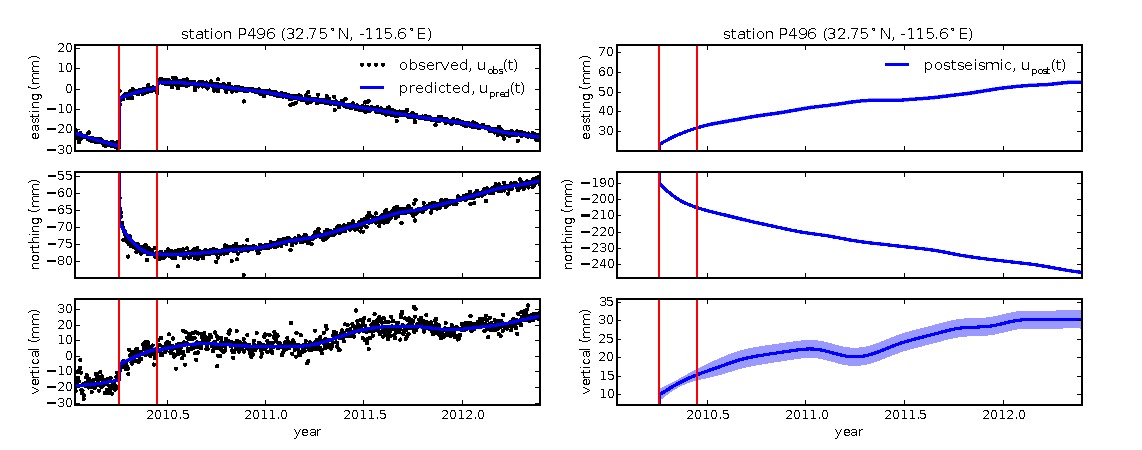
\includegraphics[scale=0.7]{Figures/FilterP496}
\centering
\caption{Left panels show GPS time series from UNAVCO (black) and the predicted displacement (blue) from eq. (\ref{TimeSeriesModel}) for a near-field station.  Red lines indicate the times of the El Mayor-Cucapah and Ocotillo earthquake. The right panels show estimated coseismic and postseismic displacements, $u_\mathrm{post}$, which are extracted from the predicted displacements.  The 68\% confidence interval is shown in light blue.}
\label{fig:P496}
\end{figure}

\begin{figure}
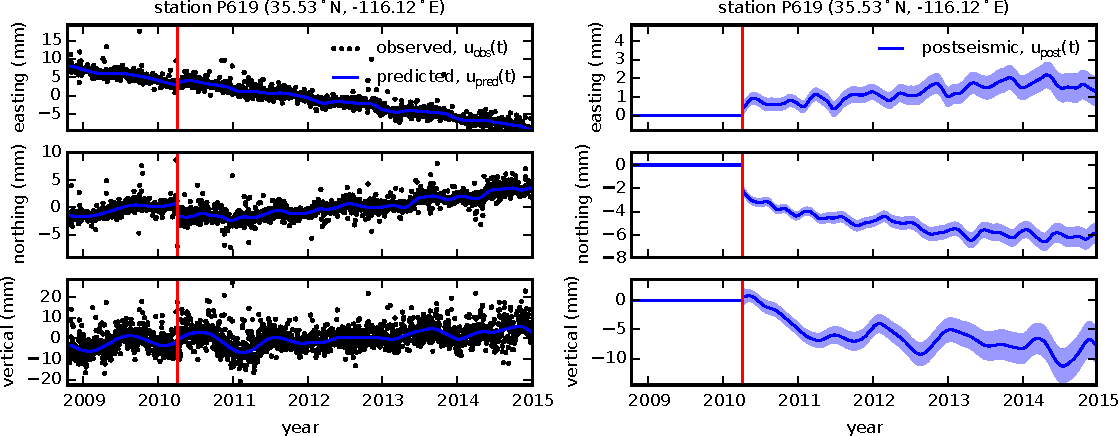
\includegraphics[scale=0.7]{Figures/FilterP619}
\centering
\caption{same as Figure \ref{fig:P496} but for a far-field station.} 
\label{fig:P619}
\end{figure}

It is important to note that the shown uncertainties in $u_\mathrm{post}(t)$ do not account for the non-negligible epistemic uncertainty in eq. (\ref{TimeSeriesModel}).  For example, we assume a constant rate of secular deformation, which appears to be an appropriate approximation for all but perhaps the stations closest to the Hector Mine epicentre, as noted above.  Also, our model for seasonal deformation in eq. (\ref{TimeSeriesModel}) assumes a constant amplitude over time, which means that any yearly variability in the climatic conditions could introduce systematic residuals \citep{Davis2012}. Indeed, it would be more appropriate to consider the seasonal amplitudes $c_2-c_5$ in eq. (\ref{TimeSeriesModel}) as stochastic variables \citep{Murray2005}. By using constant seasonal amplitudes our estimate of $u_\mathrm{post}(t)$ seems to describe some of the unmodelled annual and semi-annual oscillations (e.g. Figure \ref{fig:P619}).          

We show in Figures \ref{fig:NearField} and \ref{fig:FarField} the near and far-field postseismic displacements accumulated over the intervals  0-0.8 years, 0.8-3.0 years, and 3.0-5.0 years, as well as the coseismic displacements.  In the far-field to the north, we can see south trending displacements for the first 3 years following the earthquake at stations as far as $\sim$400 km from of the El Mayor Cucapah epicentre.  These displacements are most pronounced along the direction of the El Mayor-Cucapah P axis. A similar eastward trend can be seen in the few far-field stations along the T axis in Arizona.  After 3 years, the trend in far-field postseismic deformation is barely perceptible.  The vertical deformation in the far-field is difficult to attribute to postseismic processes.  Most far-field stations display an initial subsidence for the first year after the El Mayor-Cucapah earthquake followed by continued uplift.  This trend in vertical deformation can be observed in all three of the quadrants where postseismic data is available, which means that the vertical deformation does not exhibit an anti-symmetric quadrant pattern, as would be expected for postseismic processes.  Although we use vertical deformation in our analysis in Section \ref{sec:Model},  we do not put an emphasis on trying to describe the vertical deformation as it likely does not have postseismic origins.        

\begin{figure}
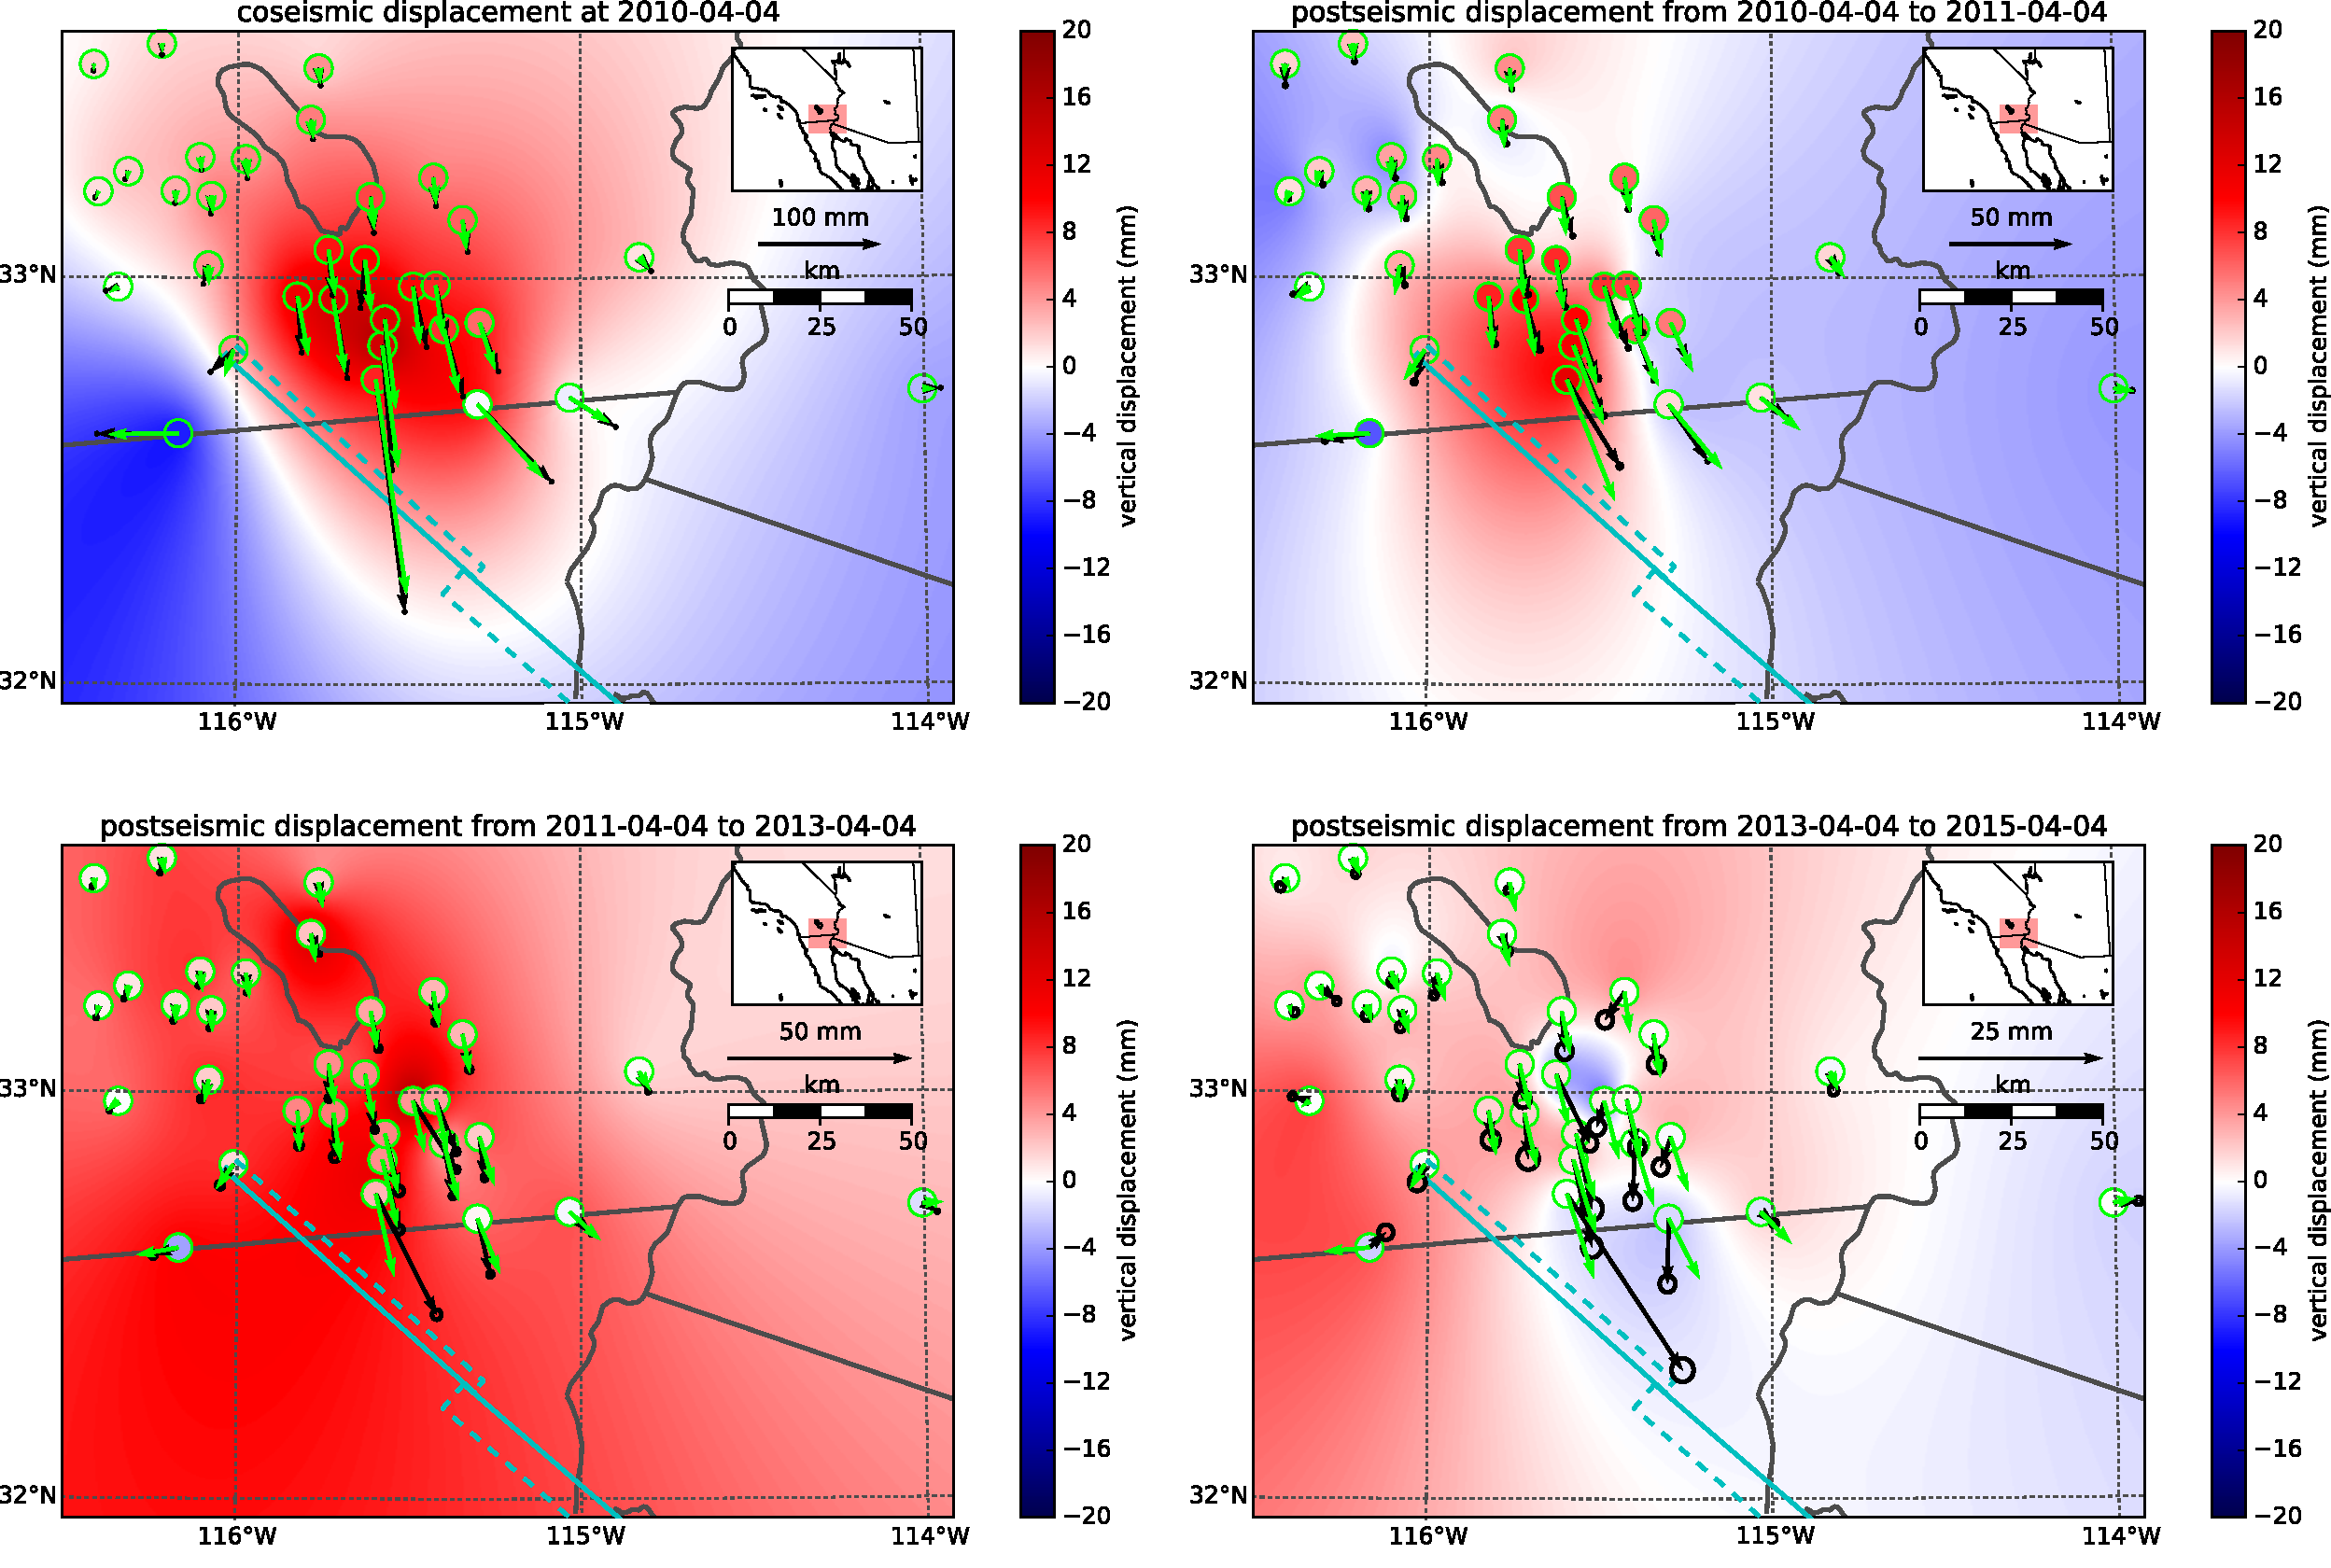
\includegraphics[scale=0.7]{Figures/MapViewNearField}
\centering 
\caption{Near-field coseismic and postseismic displacements (black) as well as predicted displacements for our preferred model from Section \ref{sec:FullInversion} (green).  Observed vertical deformation is shown as an interpolant and predicted vertical displacements are shown within the circles at the base of each vector.  Note that the interpolant is not well constrained in Mexico where there is no data available.}
\label{fig:NearField}
\end{figure}

\begin{figure}
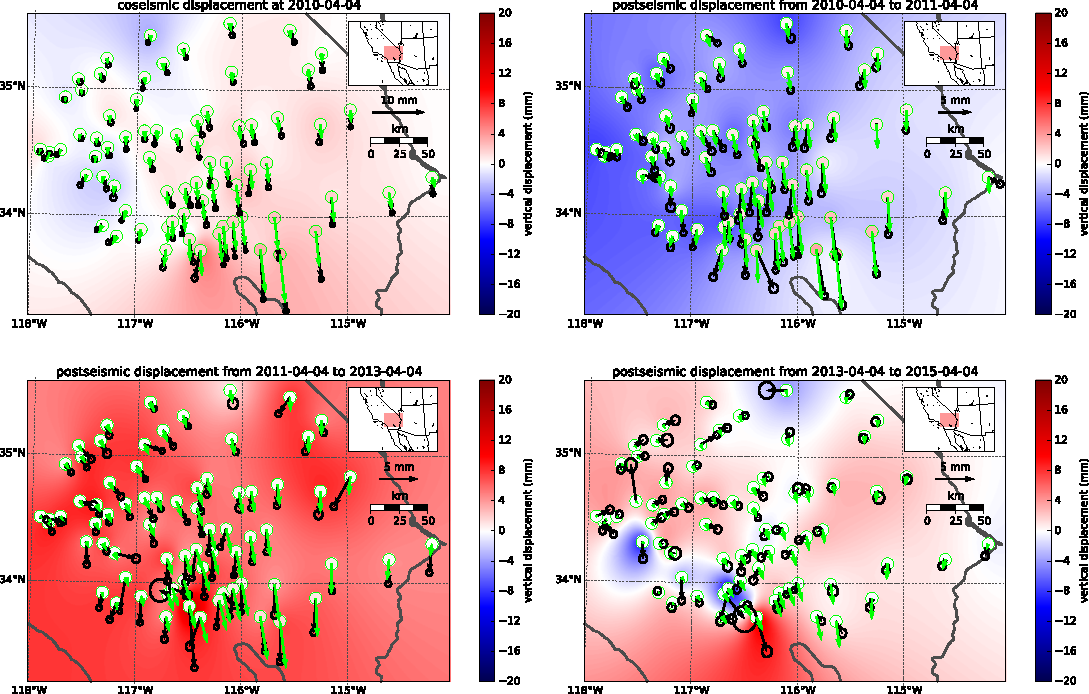
\includegraphics[scale=0.7]{Figures/MapViewFarField}
\centering 
\caption{Same as Figure \ref{fig:NearField} but for far-field stations.}
\label{fig:FarField}
\end{figure}

The near-field postseismic deformation is notably sustained when compared to the far-field deformation.  Namely, the station in this study which is closest to the El Mayor-Cucapah epicentre, P496, has been moving at a steady rate of $\sim1.5$ cm/yr to the south since $\sim1$ year after the El Mayor-Cucapah earthquake.  Vertical postseismic deformation in the near-field does display a quadrant pattern which is consistent with the coseismic vertical deformation, suggesting that it is resulting from tectonic processes.  However, the vertical postseismic signal is only apparent for the first year after the earthquake (Figure \ref{fig:NearField}).  As with the far-field deformation, there is a general trend of uplift in the near-field after $\sim1$ year, which we do not consider to be related to postseismic processes.  

%%%%%%%%%%%%%%%%%%%%%%%%%%%%%%%%%%%%%%%%%%%%%%%%%%%%%%%%%%%%%%%%%%%%%%%%%%%%%%
%%%%%%%%%%%%%%%%%%%%%%%%%%%%%%%%%%%%%%%%%%%%%%%%%%%%%%%%%%%%%%%%%%%%%%%%%%%%%%
\section{Postseismic Modeling}\label{sec:Model}

\begin{table}\label{tab:MaterialProperties}
\begin{tabular} {l l l l l}
depth (km) &$\lambda$ (GPa)&$\mu$ (GPa)&$\eta_\mathrm{eff}$ ($10^{18}$ Pa s) & $\mu_\mathrm{k}/\mu$\\ \hline
0-5 & 24.0 & 24.3 & - & -\\
5-15 & 35.2 & 35.4 & - & -\\
15-30 & 41.8 & 41.9 & 44.3 & 0.0\\
30-60 & 61.0 & 60.8 & 5.91 & 0.375\\
60-90 & 61.0 & 60.8 & 1.99 & 0.375\\
90-120 & 61.0 & 60.8 & 1.31 & 0.375\\
120-150 & 61.0 & 60.8 & 1.10 & 0.375\\
150-$\infty$ & 61.0 & 60.8 & 1.07 & 0.375\\
\end{tabular}
\caption{Assumed and estimated material properties. $\lambda$ and $\mu$ are assumed known \textit{a priori}, $\eta_\mathrm{eff}$ is estimated in Section \ref{sec:InitialInversion} and $\frac{\mu_k}{\mu}$ are the optimal shear moduli ratios found in Section \ref{sec:FullInversion} for a Zener rheology upper mantle.} 

\end{table}
In this paper, we seek to find the mechanisms driving 5 years of postseismic deformation following the El Mayor-Cucapah earthquake. We consider afterslip and viscoelastic relaxation in the lithosphere and asthenosphere as candidate mechanisms.  Poroelastic rebound has also been used to model postseismic deformation \citep[e.g.][]{Jonsson2003}; however, \citet{Gonzalez-ortega2014} suggest that any contribution to postseismic deformation from poroelastic rebound would be negligible. Furthermore, we consider stations which are sufficiently far away from the main rupture that poroelastic rebound should be insignificant.  

We estimate coseismic and time-dependent postseismic fault slip, both of which are assumed to occur on a fault geometry modified from \citet{Wei2011}.  Field studies \citep{Fletcher2014} and LIDAR observations \citep{Oskin2012} have revealed a significantly more complicated fault geometry than what was inferred by \citet{Wei2011}, especially within the Sierra Cucapah.  However, we find that a relatively simple coseismic fault geometry based on \citep{Wei2011} is adequate because most of the stations used in this study are sufficiently far from the El Mayor-Cucapah rupture zone that they are insensitive to the details in the fault geometry found by \citet{Fletcher2014} and \citet{Oskin2012}.  The fault geometry used in this study (Figure \ref{fig:ContextMap}) consists of the two main fault segments inferred by \citet{Wei2011}, where the northern segment runs through the Sierra Cucapah up to the US-Mexico border and the southern segment is the Indiviso fault which extends down to the Gulf of California. Both segments extend from the surface to 15 km depth.  We extend the northern segment by 40 km to the north-west, motivated by the clustering of aftershocks on the northern tip of the coseismic rupture zone \citep{Hauksson2011,Kroll2013}.  This extended fault segment was also found to be necessary by \citet{Rollins2015} and \citet{Pollitz2012} in order to describe the postseismic deformation. 

%%%%%%%%%%%%%%%%%%%%%%%%%%%%%%%%%%%%%%%%%%%%%%%%%%%%%%%%%%%%%%%%%%%%%%%%%%%%%%
\subsection{elastic inversion}\label{sec:ElasticInversion}    
We consider a variety of rheologic models for the lower crust and upper mantle. The simplest rheologic model is to consider them to be effectively elastic and isotropic.  In such case, the rheologic parameters consist of the Lam\'e parameters, $\lambda$ and $\mu$, which are reasonably well known and we use the values listed in Table \ref{tab:MaterialProperties} throughout this paper.  The only unknown is the distribution of fault slip, which can be easily estimated from postseismic deformation through linear least squares.  Using a subset of the GPS stations considered in this study, \citet{Rollins2015} found that postseismic deformation following the El Mayor-Cucapah earthquake can be explained with afterslip on the coseismic fault plane and they did not require any viscoelastic relaxation to describe the observations. We also perform an elastic slip inversion but we use GPS stations within a larger radius about the El Mayor-Cucapah epicentre (400 km instead of $\sim$200 km). Our forward problem describing predicted postseismic deformation, $u_\mathrm{pred}$, in terms of time dependent fault slip, $s$, is
\begin{equation}\label{eq:ElasticForward}
  u_\mathrm{pred}(x,t) = \int_F s(\xi,t)g(x,\xi)d\xi 
\end{equation}           
where $g(x,\xi)$ is elastic Green's function describing displacement at surface position $x$ resulting from a unit of slip at $\xi$ on the fault, which is denoted by $F$.  We estimate coseismic slip and the rate of afterslip at the discrete time intervals, 0.0-0.125, 0.125-0.25, 0.5-1.0, 1.0-2.0, 2.0-3.0, 3.0-4.0, and 4.0-5.0 years after the earthquake.  Each fault segment is discretized into roughly 4 km by 4 km patches and we estimate a strike-slip and thrust component of slip for each patch. We impose that the direction of slip and slip rate are within 45$^\circ$ of right-lateral. We also add zeroth order Tikhonov regularization so that our solution for $s$ satisfies
\begin{equation}\label{eq:ElasticObjective}
  \min_s \left(\left|\left|\frac{u_\mathrm{pred}(s) - u_\mathrm{post}}                
                                {\sigma_\mathrm{obs}}\right|\right|_2^2 + 
                                \lambda_s||s||_2^2\right). 
\end{equation}
The penalty parameters, $\lambda_s$, is chosen with a trade-off curve.  We use Pylith \citep{Aagaard2009} to compute the Green's functions for this inversion and for the remaining inversions in this paper. 

Our coseismic slip and afterslip solutions are shown in Figure \ref{fig:ElasticSlip}.  As with \citet{Rollins2015}, we find that a large amount of afterslip on the southern fault segment is required to explain the observations. The potency of our inferred coseismic slip is $3.2\times10^9\ \mathrm{m}^3$, equivalent to a Mw7.28 earthquake when assuming a shear modulus of 32 GPa.  The potency of our inferred cumulative 5 years of afterslip is $6.1\times10^9\ \mathrm{m}^3$, equivalent to a Mw7.46 earthquake, which is unrealistically large if we consider afterslip to be driven by coseismically induced stresses.  Our elastic slip model accurately describes near-field postseismic deformation, while it systematically underestimates postseismic deformation for stations further than $\sim150$ km from the El Mayor-Cucapah epicentre (Figure \ref{fig:RecordSectionElastic}).  When the fault segments used in the inversion are extended down to 30 km depth, rather than 15 km, the systematic far-field residuals are smaller but remain apparent. Because an elastic model for the lithosphere requires an unrealistic amount of afterslip and is unable to predict far-field deformation, we move on to consider viscoelastic models in the next section.  

\begin{figure}
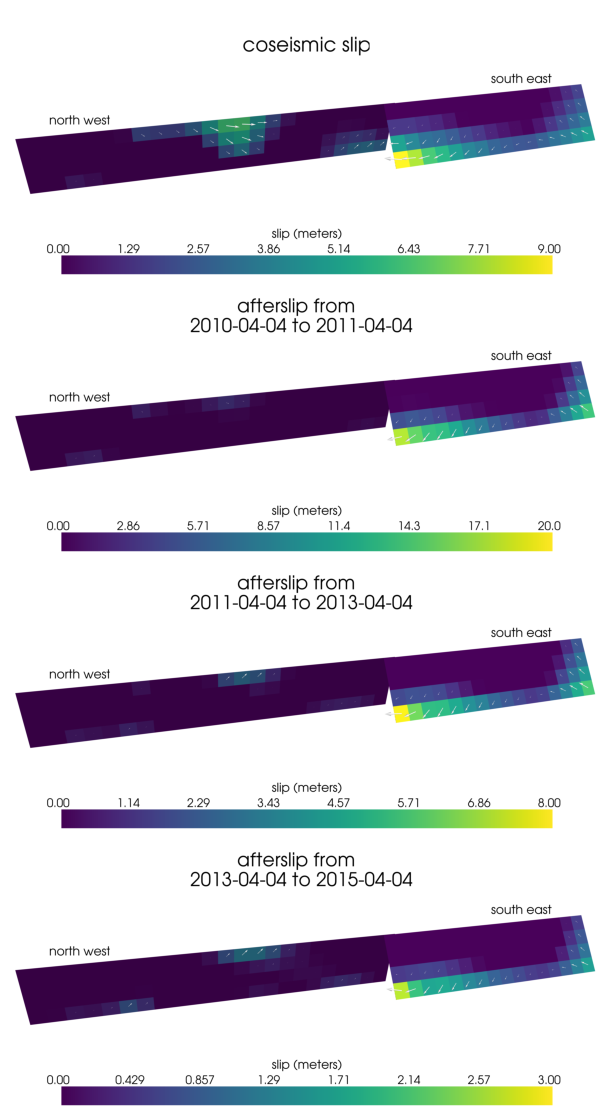
\includegraphics[scale=0.7]{Figures/ElasticSlip}
\caption{Coseismic slip and cumulative afterslip over the indicated intervals for the elastic model from Section \ref{sec:ElasticInversion}.  Color indicates the magnitude of slip while arrows indicate the motion of the hanging wall.}
\label{fig:ElasticSlip}
\end{figure}

\begin{figure}
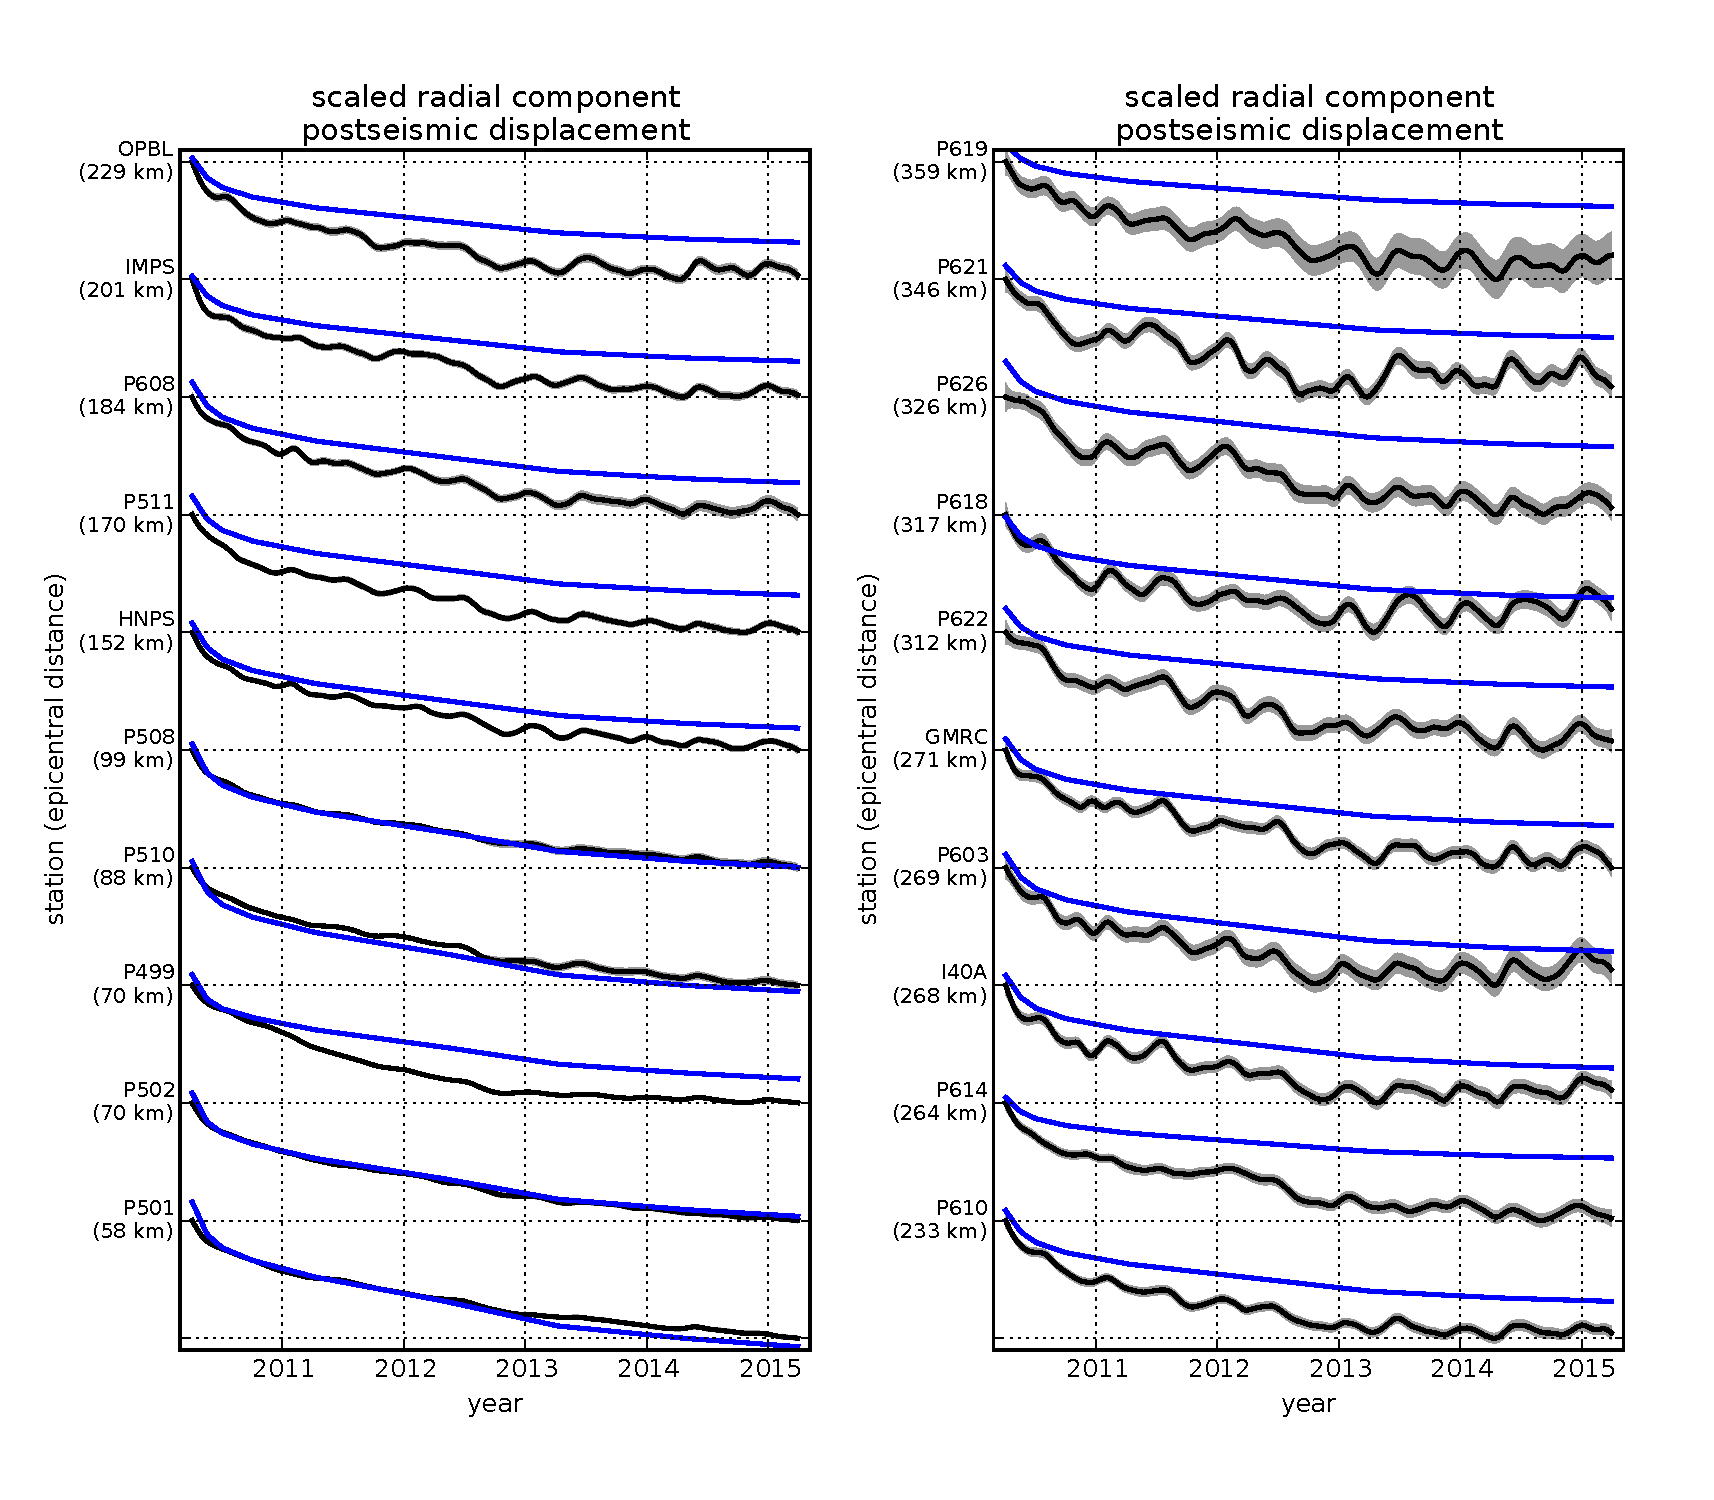
\includegraphics[scale=0.7]{Figures/RecordSectionElastic}
\caption{Scaled record section for the radial component of observed postseismic displacements, $u_\mathrm{obs}$ (black) and displacements predicted by an elastic model, $u_\mathrm{pred}$ (blue).  Downward motion indicates that the station is moving toward the El Mayor-Cucapah epicentre.  Displacement time series are scaled so that the minimum and maximum observed values lie on the grid lines. The standard deviation of observed displacements are shown in gray.}
\label{fig:RecordSectionElastic}
\end{figure}

%%%%%%%%%%%%%%%%%%%%%%%%%%%%%%%%%%%%%%%%%%%%%%%%%%%%%%%%%%%%%%%%%%%%%%%%%%%%%%
\subsection{constraints on effective viscosity}\label{sec:InitialInversion}


For any linear viscoelastic rheology of the crust and mantle, postseismic displacements resulting from time dependent fault slip can be described as  
\begin{equation}\label{GeneralForward}
  u_\mathrm{pred}(x,t) = \int_F s(\xi,t)g(x,\xi)d\xi + 
           \int_0^t\int_F s(\xi,\tau) f(t-\tau,x,\xi) d\xi d\tau
\end{equation}
where $f(t,x,\xi)$ describes the time-dependent velocity at $x$ resulting from viscoelastic relaxation of stresses induced by slip at $\xi$. $f$ is a function of $\lambda$, $\mu$, and any additional rheologic parameters controlling the viscoelastic response, which are generally not well known. Schematic representations of the viscoelastic rheologic models considered in this study are shown in Figure \ref{fig:Rheology}.  We consider Maxwell viscoelasticity, where the steady-state viscosity, $\eta_M$, is unknown, Zener viscoelasticty, where the transient viscosity, $\eta_K$, and transient shear modulus, $\mu_K$, are unknown, and Burgers viscoelasticity, where $\eta_M$, $\eta_K$, and $\mu_K$, are all unknown. We further discuss these rheologic models and their use in geophysical studies in Section \ref{Discussion}. 

\begin{figure}
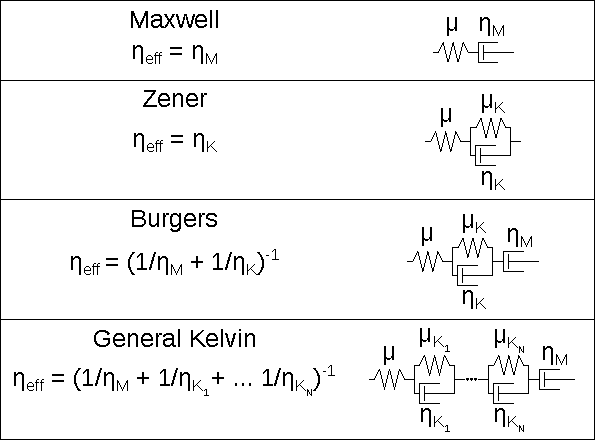
\includegraphics[scale=0.7]{Figures/rheology}
\centering 
\caption{Schematic illustration of rheologic models considered in this paper as well as their initial effection viscosities, $\eta_\mathrm{eff}=\frac{\sigma}{\dot\epsilon}|_{t=0}$.}
\label{fig:Rheology}
\end{figure}

In order to greatly simplify the inverse problem, we use the method described in \citet{Hines2015} to constrain an initial effective lithospheric viscosity structure from the early postseismic deformation.  The method relies upon the fact that immediately after an earthquake, stresses throughout the crust and mantle are only controlled by the relatively well known instantaneous elastic properties and each parcel will have a strain rate, $\dot\epsilon$, that is proportional to stress, $\sigma$, and inversely proportional to the parcel's effective viscosity, $\eta_{\mathrm{eff}}=\frac{\sigma}{\dot{\epsilon}}|_{t=0}$. Through linear superposition, we can deduce that the initial rate of surface deformation resulting from viscoelastic relaxation is a summation of the surface deformation resulting from each parcel, scaled by the reciprocal of the parcel's effective viscosity. That is to say   
\begin{equation}\label{InitialRate}
  f(0,x,\xi) = \int_L \frac{h(x,\xi,\zeta)}{\eta_\mathrm{eff}(\zeta)} d\zeta, 
\end{equation}
where $h(x,\xi,\zeta)$ describes the initial rate of deformation resulting from viscoelastic relaxation at $\zeta$ induced by slip at $\xi$ and $L$ denotes the crust and mantle. We can combine eq. (\ref{InitialRate}) with eq. (\ref{GeneralForward}) to get a first order approximation for early postseismic deformation,
\begin{equation}\label{ApproxForward}
  u_\mathrm{pred}(x,t) \approx \int_F s(\xi,t)g(x,\xi)d\xi + 
           \int_0^t\int_F\int_L \frac{s(\tau,\xi)}{\eta_\mathrm{eff}(\zeta)} h(x,\xi,\zeta) d\zeta d\xi d\tau,
\end{equation}
which is valid for as long as the rate of deformation resulting from viscoelastic relaxation is approximately constant. Although eq. (\ref{ApproxForward}) may only be valid for a short portion of the postseismic period, its utility becomes apparent when noting that $g$ and $h$ are only functions of the fault geometry and instantaneous elastic properties, $\lambda$ and $\mu$, and so $g$ and $h$ can be computed numerically as a preprocessing step and the forward problem in eq. (\ref{ApproxForward}) can be rapidly evaluated for any realization of $s$ and $\eta_{\mathrm{eff}}$.  This is in contrast to evaluating the full forward problem, eq. (\ref{GeneralForward}), numerically for each realization of $s$ and unknown rheologic properties. Figure \ref{fig:Rheology} shows how estimates of $\eta_\mathrm{eff}$ can then be used as a constraint on the unknown parameters for various linear viscoelastic rheologies.    

We perform an initial inversion of postseismic displacements using the approximation in eq. (\ref{ApproxForward}).  We estimate coseismic slip and afterslip with the same spatial and temporal discretization as in Section \ref{sec:ElasticInversion}. Simultaneously, we estimate $\eta_{\mathrm{eff}}$ within six vertically stratified layers which have depths ranging from 15-30 km, 30-60 km, 60-90 km, 90-120 km, 120-150 km, as well as from 150 km to the bottom of our numerical model domain at 800 km.  We again restrict fault slip to occur between 0 and 15 km depth and we made this choice to help eliminate inevitable non uniqueness.  It has long been recognized that fault slip at sufficiently great depths can produce surface deformation that is indistinguishable from viscoelastic relaxation, at least in two-dimensional earthquake models \citep{Savage1990}. Since we are trying to simultaneously model these two processes, it is necessary to put sensible constraints on the depth of fault slip.  Additionally, we note that when simultaneously estimating afterslip in the lower crust and a lower crustal viscosity, the inverse problem becomes particularly ill-posed. This ill-posedness is illustrated in Figure (\ref{fig:LowerCrust}), which shows the displacements resulting from a meter of slip on a fault extending from 15 to 30 km depth and the initial velocity resulting from viscoelastic relaxation in the lower crust, which is given a viscosity of $10^{18}$ Pa s.  The horizontal displacements from fault slip are in the opposite direction as the displacements resulting from subsequent viscoelastic relaxation.  This means that surface displacements resulting from afterslip at lower crustal depths can be cancelled out, at least partially, by a low viscosity lower crust.  We eliminate this null space by allowing only one mechanism in the lower crust, which we choose to be viscoelastic relaxation.  This is not to say that we do not believe deep afterslip to be a possibility, rather we restrict slip to seismogenic depths as a modelling necessity. Although, it has been noted that the pattern of vertical postseismic deformation following the El Mayor-Cucpah earthquake indicates that a significant amount of afterslip must be shallow \citep{Rollins2015}.  
 
\begin{figure}
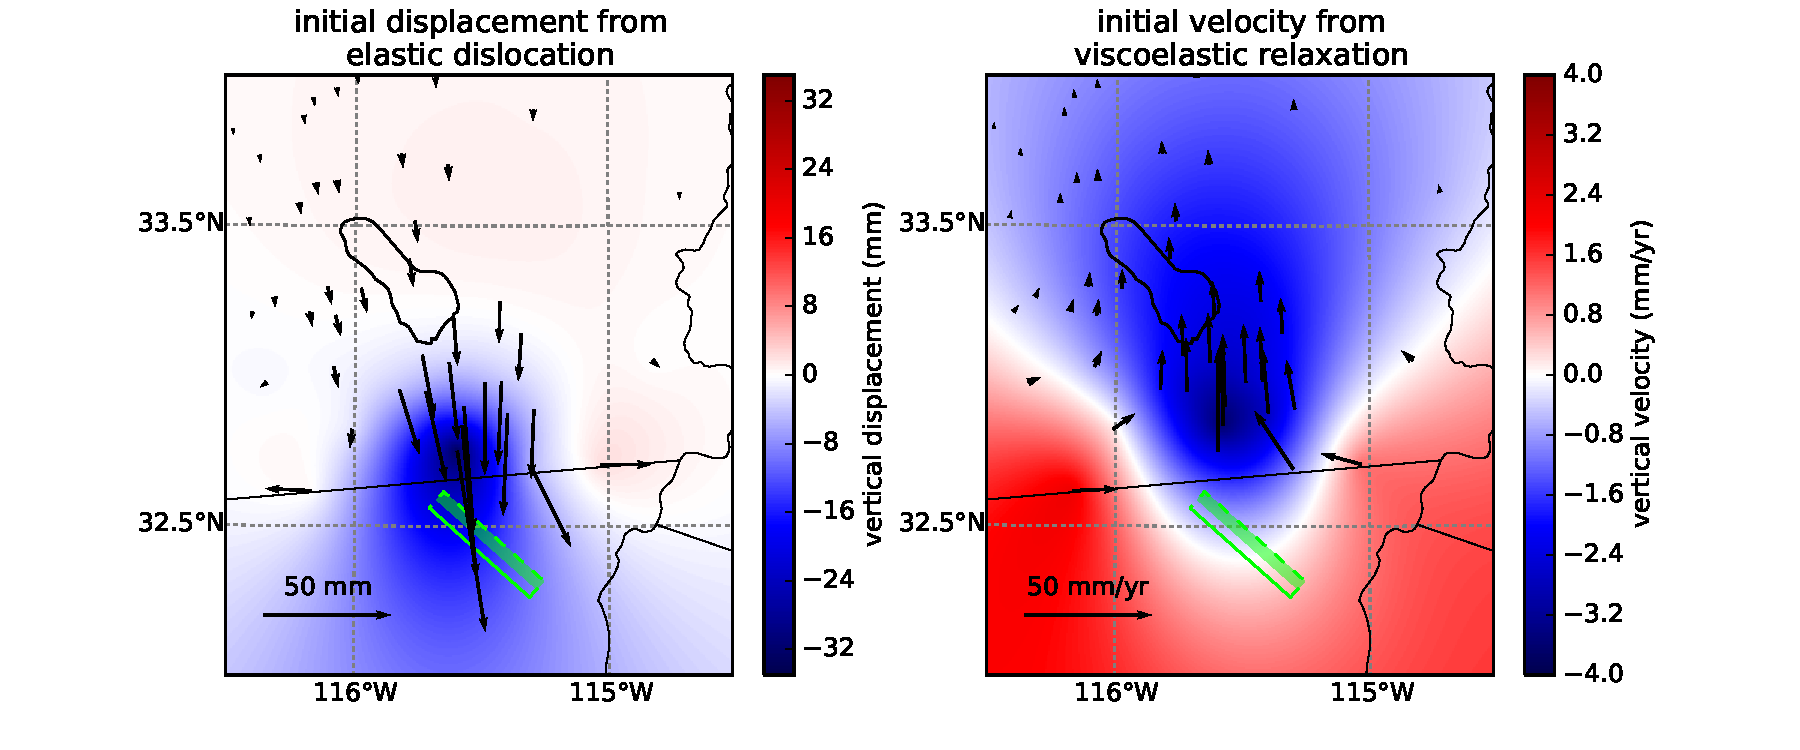
\includegraphics[scale=0.5]{Figures/Cancellation}
\caption{Displacements resulting from fault slip at lower crustal depths (left), and initial velocity resulting from subsequent relaxation of a viscoelastic lower crust (right).  The fault segment dips $75^\circ$ to the north east and its surface projection is outlined in green.  The highlighted area on the fault extends from 15 to 30 km depth and indicates where 1 meter of right-lateral slip was imposed.  The elastic properties of the crust and mantle are the same as in Table \ref{tab:MaterialProperties} and $\eta_\mathrm{eff}=10^{18}$ Pa s in the lower crust.  Vertical dispalcements are interpolated between station locations.}
\label{fig:LowerCrust}
\end{figure}
 
Further details on how $s$ and $\eta_\mathrm{eff}$ are estimated from postseismic deformation can be found in \citet{Hines2015}. A non-linear Kalman filter based inverse method can also be used to estimate $s$ and $\eta_{\mathrm{eff}}$ in a manner akin to \citet{Segall1997} or \citet{McGuire2003}, in which we would not have to explicitly impose a time dependent parametrization of $s$. We have thoroughly explored Kalman filter based approaches, but we ultimately prefer the method described in \citet{Hines2015} because of its relative simplicity. Moreover, we believe the piecewise continuous representation of slip with respect to time to be sufficiently general for the resolving power of these GPS data.

The first step in our inverse method is to determine at which point the early postseismic approximation breaks down, which we will denote as $t_{\mathrm{bd}}$.  As noted, it is valid for approximately as long as the rate of deformation resulting from viscoelastic relaxation is approximately constant. We can almost certainly assume that deformation at the most far-field stations, which are $\sim400$ km away from the El Mayor-Cucapah epicentre, is the result of viscoelastic relaxation. The approximation should then be valid for as long as a linear trend adequately approximates the far-field deformation. Using this logic, it would appear that $t_{\mathrm{bd}}\approx1$ year after the El Mayor-Cucapah earthquake.  Another way to determine $t_{\mathrm{bd}}$ is to find the best fitting prediction of eq. (\ref{ApproxForward}) to observed deformation using increasing durations of the postseismic time series.  $t_\mathrm{bd}$ should be the point when eq. (\ref{ApproxForward}) is no longer capable of describing the observed deformation without incurring systematic misfits.  This is illustrated in Figure \ref{fig:RecordSection1}, which show the scaled radial components of displacement for stations along the El Mayor-Cucapah P axis.  When using eq. (\ref{ApproxForward}) to fit the entire 5 years of postseismic displacement we see that the near-field displacements, e.g. station P501, are accurately predicted but when looking at displacement in the far-field, e.g. station P621, we see that eq. (\ref{ApproxForward}) overestimates the rate of deformation in the later postseismic period and underestimates the rate of deformation in the early period.  Due to the low signal-to-noise ratios for far-field stations, it is difficult to determine at what point eq. (\ref{ApproxForward}) is no longer able to predict the observed displacements without incurring any significant systematic misfit; however, we settle on $t_{\mathrm{bd}}=0.8$ years after the earthquake, while acknowledging that the choice is subjective. As noted in \citet{Hines2015}, overestimating $t_{\mathrm{bd}}$ will result in a bias towards overestimating $\eta_{\mathrm{eff}}$, while picking a $t_\mathrm{bd}$ which is too low will not necessarily result in a biased estimate of $\eta_\mathrm{eff}$, although the uncertainties would be larger. We can then consider inferences of $\eta_{\mathrm{eff}}$ to be an upper bound on the viscosity needed to describe the far-field rate of deformation during the first 0.8 years of postseismic deformation. 

\begin{figure}
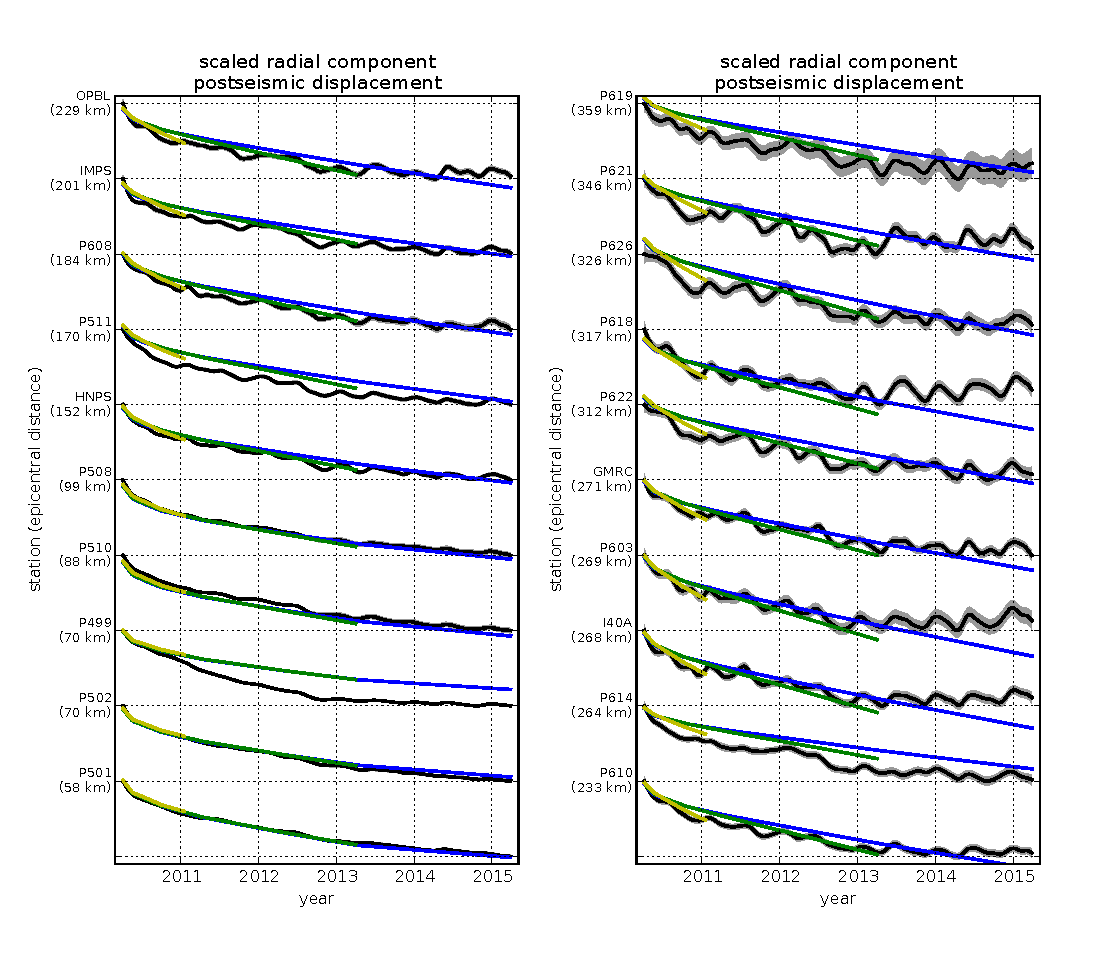
\includegraphics[scale=0.7]{Figures/RecordSectionDuration}
\centering 
\caption{Illustration of how $t_\mathrm{bd}$ is chosen. Observed postseismic displacements are shown in black.  Blue, green and yellow lines are the best fitting predictions to 5.0, 3.0, and 0.8 years of the postseismic data, respectively, from eq. \ref{ApproxForward}.}  
\label{fig:RecordSection1}
\end{figure}

We estimate coseismic slip, afterslip, and effective viscosity by solving 
\begin{equation}\label{ObjectiveFunction}
 \mathrm{min}_{s,\eta_\mathrm{eff}} \left(\left|\left|
 \frac{u_\mathrm{pred}(s,\eta_\mathrm{eff}) - u_\mathrm{obs}}
 {\mathbf{\sigma_\mathrm{obs}}}\right|\right|_2^2 + 
 \lambda_s||s||_2^2 + 
 \lambda_\eta||\nabla \eta_{\mathrm{eff}}^{-1}||_2^2\right)
\end{equation} 
where $u_\mathrm{obs}$ consists of the first 0.8 years of postseismic deformation and $u_\mathrm{pred}$ are the predicted displacements from eq. (\ref{ApproxForward}).  Due to inherent non uniqueness, we have added zeroth order Tikhonov regularization to estimates of $s$, and second order Tikhonov regularization to estimates of effective fluidity, $\eta_\mathrm{eff}^{-1}$. The degree to which we impose the regularization on slip and fluidity is controlled by the penalty parameters $\lambda_s$ and $\lambda_\eta$.  The penalty parameters are chosen with two trade-off curves. We first choose $\lambda_s$ while fixing $\lambda_\eta$ at 0 and then we determine $\lambda_\eta$ with $\lambda_s$ fixed at its chosen value. Our goal here is to get a prior constraint on $\eta_{\mathrm{eff}}$ to minimize the amount of searching we have to do when describing the postseismic deformation over the full 5 years, which we do in Section \ref{sec:FullInversion}.  Estimates of $s$ made here will not be used in Section \ref{sec:FullInversion}, and so the motivation behind even adding regularization to $s$ is to ensure that the slip driving viscoelastic relaxation in eq. (\ref{ApproxForward}) is sensible.  

Our inferred estimates of effective viscosities, and corresponding fluidities, are shown in Figure \ref{fig:EffectiveViscosity} with their 95\% confidence intervals indicated, which were estimated through bootstrapping. Although fluidity is rarely used in geophysical literature, eq. (\ref{InitialRate}) is linear with respect to fluidity and so the fluidity indicates the amplitude of the viscoelastic signal coming from each layer.  We note that the magnitude of the uncertainties on viscosity tend to decrease as we increase $\lambda_\eta$. Our choice of $\lambda_\eta$ was based on a standard technique used in geophysical inverse problems which has no statistical backing.  It is therefore difficult to interpret the magnitude of uncertainties on viscosities shown in Figure \ref{fig:EffectiveViscosity}; although, we do believe that the relative uncertainty between layers is accurately depicted. A robust feature that we see is that the largest jump in fluidity is at 60 km depth, which is consistent with the range of lithosphere-asthenosphere boundary depths inferred by \citet{Lekic2011}. This transitional depth is also consistent with the the viscosity structure required to explain far field postseismic deformation following the Hector Mine earthquake \citep{Freed2007a}. We find that the viscosity below 60 km depth needs to be $\sim1\times10^{18}$ Pa s to describe the early rate of postseismic deformation at far-field stations while the lower crust and uppermost mantle need to be relatively stronger.  The viscosity of the lower crust is the least well constrained as there is no evidence of relaxation in that layer, meaning that it is effectively elastic over the first 0.8 years after the earthquake.  

\begin{figure}
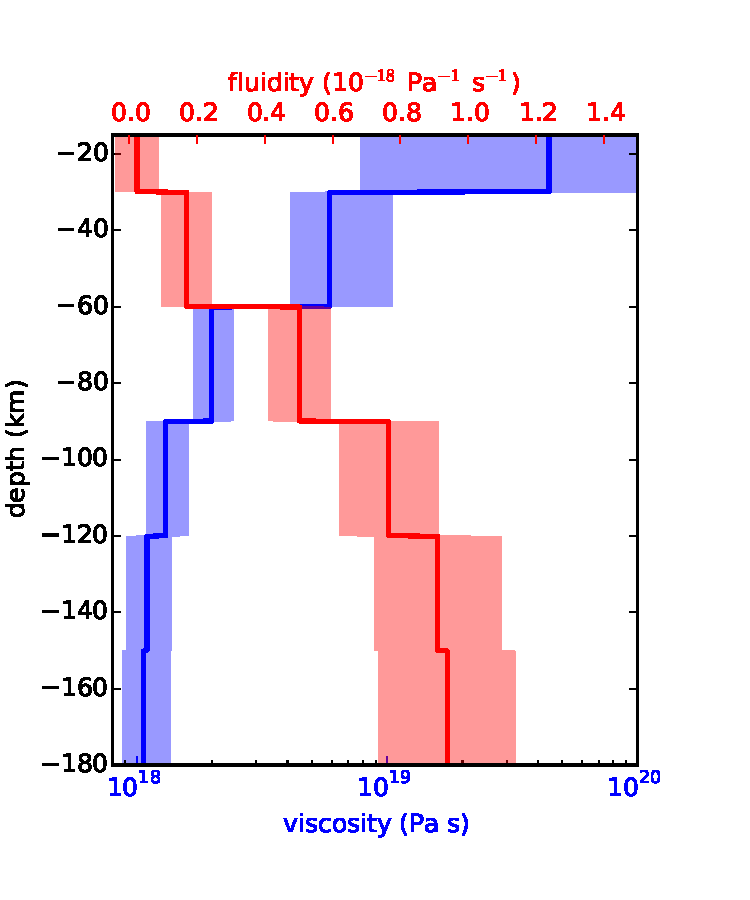
\includegraphics[scale=0.7]{Figures/EffectiveViscosity}
\centering 
\caption{Effective viscosity and associated fludities inferred by fitting eq. (\ref{ApproxForward}) to the first 0.8 years of postseismic displacements. 95\% confidence intervals, estimated from bootstrapping, are also shown.}
\label{fig:EffectiveViscosity}
\end{figure} 

Our initial estimate for coseismic slip and cumulative afterslip over the first 0.8 years after the El Mayor-Cucapah earthquake are shown in Figure \ref{fig:InitialSlip}.  Similar to our elastic slip model from Section \ref{sec:ElasticInversion}, coseismic slip is inferred to be in the Sierra Cucapah and it is right lateral with a significant normal component.  This is consistent with field studies \citep{Fletcher2014}, as well as the coseismic slip from \citet{Wei2011}. The potency of inferred coseismic slip is $3.3\times 10^{9}\ \mathrm{m}^3$, which is also about the same as that inferred from Section \ref{sec:ElasticInversion}. The present inference of afterslip on the Indiviso fault is significantly less than what was found in the Section \ref{sec:ElasticInversion} where we did not account for viscoelasticity. When fault slip is simultaneously estimated with a lithospheric and asthenospheric viscosity, the potency of inferred afterslip over the first 0.8 years after the earthquake is $0.85\times 10^9\ \mathrm{m}^3$, compared to $3.46\times10^{9}\ \mathrm{m}^3$ when we assume the lithosphere and asthenosphere are elastic.  The significant amount of afterslip inferred on the Indiviso fault seems to be compensating for unmodelled viscoelastic relaxation at depths greater than $60$ km.  The fact that there is still an appreciable amount of afterslip inferred on the Indiviso fault even when allowing for viscoelastic relaxation in the lower crust and upper mantle raises the question of whether it is compensating for viscoelastic relaxation that is more localized than what we allow for since we only estimate depth dependent variations in viscosity.  

\begin{figure}
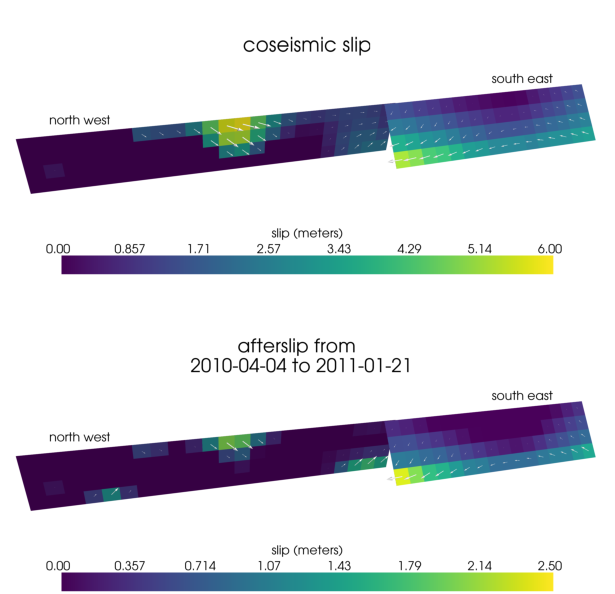
\includegraphics[scale=0.7]{Figures/InitialSlip}
\caption{Coseismic slip and afterslip inferred by fitting eq. (\ref{ApproxForward}) to the first 0.8 years of postseismic displacements.}
\label{fig:InitialSlip}
\end{figure} 

%%%%%%%%%%%%%%%%%%%%%%%%%%%%%%%%%%%%%%%%%%%%%%%%%%%%%%%%%%%%%%%%%%%%%%%%%%%%%%
\subsection{Full Inversion}\label{sec:FullInversion} 

In the previous section, we used the inverse method from \citet{Hines2015} to constrain the effective viscosity structure required to explain the first 0.8 years of postseismic deformation. In this section, we use the effective viscosities inferred above as a prior constraint when searching for models which are capable of describing the available 5 years of postseismic data, where our forward problem is now eq. (\ref{GeneralForward}) rather than the approximation given by eq. (\ref{ApproxForward}).  We perform a series of coseismic slip and afterslip inversion assuming a variety of rheologies for the lower crust and upper mantle which are consistent with our findings from Section \ref{sec:InitialInversion}.  We appraise each model using the mean chi squared value,
\begin{equation}\label{eq:Misfit}
  \bar\chi^2 = \frac{1}{N}\left|\left|\frac{u_\mathrm{pred} - u_\mathrm{obs}}{\sigma_\mathrm{obs}}\right|\right|_2^2,
\end{equation}
where $N$ is the number of observations.

We first assume that the crust and mantle can be described with a Maxwell rheology, and we set $\eta_\mathrm{M}$ equal to our inference of $\eta_{\mathrm{eff}}$.  We compute $f$ and $g$ from eq. (\ref{GeneralForward}) using the finite element software, Pylith \citep{Aagaard2009}, and assume the same spatial and temporal discretization of $s$ as in Sections \ref{sec:ElasticInversion} and \ref{sec:InitialInversion}. We estimate $s$ using linear least squares and we find $\bar\chi^2=37.4$. For comparison, $\bar\chi^2=35.3$ for the elastic model from Section \ref{sec:ElasticInversion}.  The Maxwell viscoelastic model has a larger misfit because it tends to overestimate the rate of deformation after about 3 years \ref{fig:RecordSection2}. Since our initial estimates of $\eta_\mathrm{eff}$ may be biased towards overestimating viscosities, we have also performed the slip inversion where we use uniformly lower viscosities in the crust and mantle. However, decreasing the viscosity only increases the misfit.  Although, the viscosities used here are consistent with the successful Maxwell viscoelastic models found by \citet{Rollins2015} and \citet{Spinler2015}, which had mantle viscosities on the order of $10^{18}$ Pa s, we find that such a model is incapable of describing the entire postseismic time series.  \citet{Pollitz2001} similarly recognized this deficiency in a Maxwell rheology, which then motivated their exploration of a Burgers rheology upper mantle \citep{Pollitz2003}.  

Rather than exploring a Burgers rheology mantle, which introduces two new parameters that need to be estimated, $\eta_{K}$ and $\mu_{K}$, we first consider a Zener rheology for the mantle, which only introduces the unknown parameter $\mu_{K}$.  We assume that the lower crust still has a Maxwell rheology. The steady-state viscosity, $\eta_{M}$, in the crust and the transient viscosity, $\eta_\mathrm{K}$, in the mantle are set equal to the inferred effective viscosities.  We then estimate the ratio of shear moduli, $\frac{\mu_K}{\mu}$. We compute nine different sets of Green's functions, $f$ and $g$, using Pylith, where we assume values of $\frac{\mu_K}{\mu}$ ranging from 0 to 1. The former being a degenerate case where the Zener model reduces to the above Maxwell model.  We estimate coseismic slip and afterslip for each realization of $\frac{\mu_K}{\mu}$.  The shear moduli ratio that yields to best prediction to the observed postseismic displacements is found to be $0.375$ with a misfit of $\bar\chi^2=31.2$ (Figure \ref{fig:ShearModulusRatio}).  The improvement in the Zener model over the Maxwell model can be clearly seen in the fit to the far-field data (Figure \ref{fig:RecordSection2}). The Zener model does a significantly better job at explaining the transient rate of far-field deformation throughout the 5 years.  

\begin{figure}
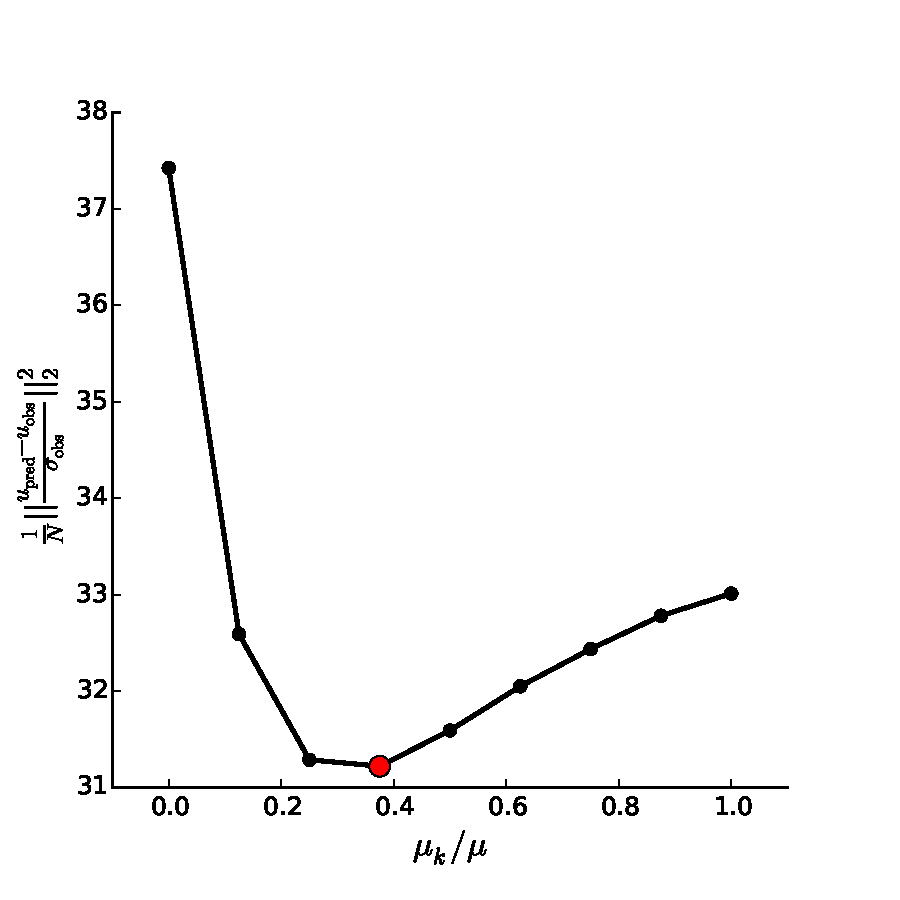
\includegraphics[scale=0.8]{Figures/RatioMisfit}
\centering 
\caption{Misfit as a function of the transient shear modulus in a Zener rheology upper mantle.}
\label{fig:ShearModulusRatio}
\end{figure}

\begin{figure}
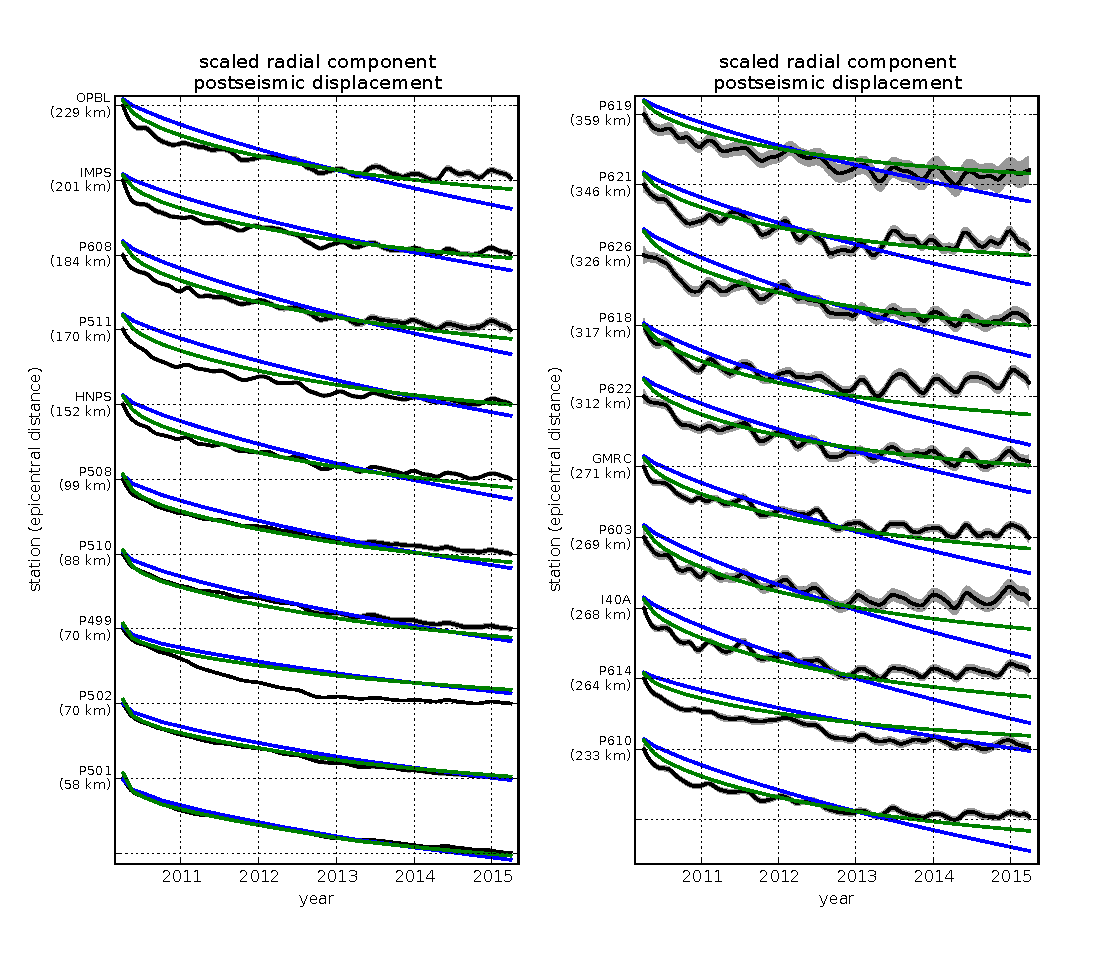
\includegraphics[scale=0.8]{Figures/RecordSectionFinal}
\centering 
\caption{Observed postseismic displacements (black) and predicted postseismic displacements for the best fitting slip models when using a Maxwell (blue) and Zener (green) rheology in the upper mantle.  The effective viscosities are the same for both models and are shown in Figure \ref{fig:EffectiveViscosity}.}
\label{fig:RecordSection2}
\end{figure} 

Because we are able to adequately describe the available 5 years of postseismic deformation with a Zener model, we do not find it necessary to explore the parameter space for a more complicated Burgers rheology.  However, since the Zener model is a Burgers model with an infinite steady-state viscosity, we can conclude that any Burgers rheology that has a transient viscosity consistent with that found in Section \ref{sec:InitialInversion} and a steady-0state viscosity of $\gtrsim10^{20}$ Pa s, which is effectively infinite on the time scale of 5 years, would also be able to satisfactorily describe the observable postseismic deformation.        
  
The regularized inference of coseismic slip and afterslip for our preferred Zener model is shown in Figure \ref{fig:FinalSlip} and the predicted postseismic displacements are shown Figures \ref{fig:NearField}, \ref{fig:FarField} and \ref{fig:RecordSection2}.  Overall, the trends in the near-field and far-field transient deformation are accurately described by our preferred model.  In particular, the trends in far-field deformation are much better described by our preferred Zener model than either an elastic model or a model with a Maxwell viscoelastic mantle (Figure \ref{fig:RecordSection2}).  There are a few areas where we have notable misfit.  Most of our misfit is for the near-field stations in the Imperial Valley, and we attribute this misfit to our relatively simple fault geometry, which does not account for potential fault slip in the Imperial Valley triggered by the El Mayor-Cucapah earthquake \citep{Wei2011a,Wei2015}. In particular, we are unable to model the sustained rapid rate of deformation at station P496, which suggests that this station could be influenced by a more localized deformation mechanism than is considered in this study.
Additionally, we see systematic misfit in the later postseismic period west of the location of the Landers and Hector Mine earthquakes, which may be the result of unmodelled postseismic deformation resulting from those earthquakes.  Lastly, there are clear discrepancies between the observed and predicted vertical deformation following the first year after the El Mayor Cucapah earthquake. We observe a broad uplift throughout Southern California, which is inconsistent with any postseismic model.

\begin{figure}
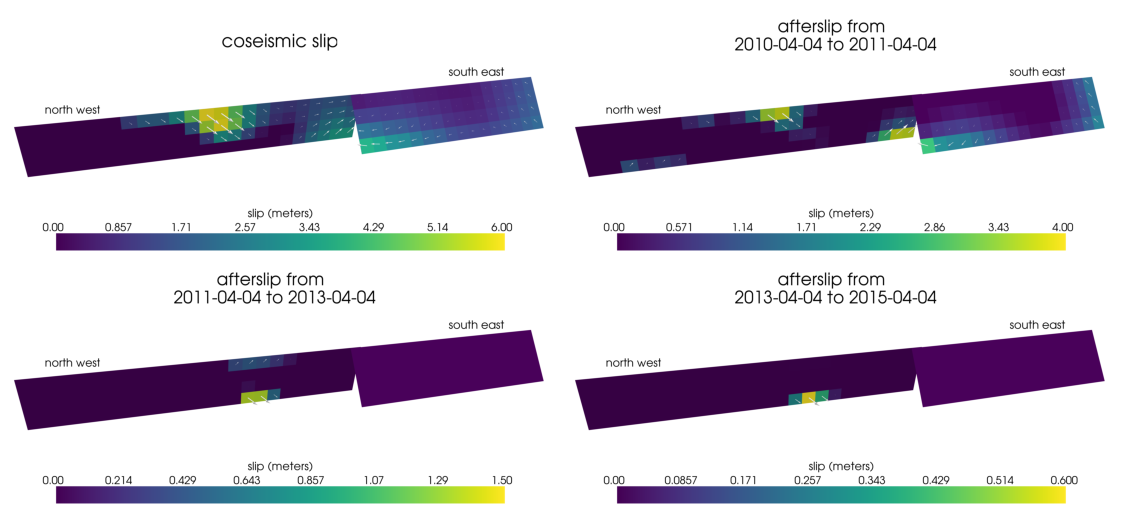
\includegraphics[scale=0.8]{Figures/FinalSlip}
\centering 
\caption{Inferred coseismic slip and afterslip when assuming a Maxwell rheology in the lower crust and a Zener rheology in the upper mantle.  $\eta_K$ in the mantle and $\eta_M$ in the crust are set equal to the effective viscosities from Figure \ref{fig:EffectiveViscosity}. We use $\frac{\mu_K}{\mu}=0.375$ in the upper mantle.}
\label{fig:FinalSlip}
\end{figure}

The inferred coseismic potency is $3.0\times10^{9}\ \mathrm{m}^3$, equivalent to a Mw7.26 earthquake, and the potency of 5 years of afterslip is $1.1\times10^{9}\ \mathrm{m}^3$. Most of the afterslip in our preferred model occurs within the first year after the earthquake with a significant amount inferred to be shallow and in the Sierra Cucapah.  The afterslip within the first year is accounting for the most rapid near-field transient deformation. After 1 year, afterslip is inferred to be deeper and under the Sierra Cucapah, which is describing much of the sustained near-field postseismic deformation.  We emphasize, that the GPS station closest to our inferred afterslip, P496, is still about 30 km away, which is too far away for us to conclusively argue for sustained brittle deformation rather shallow ductile deformation. The deep afterslip inferred after 1 year could potentially be describing deformation resulting from lower crustal flow. To test this, we have modified our preferred model by decreasing the lower crustal viscosity from $5.91\times10^{19}$ Pa s to $1\times10^{19}$ Pa s, which is still consistent with our viscosity inference from Section \ref{sec:InitialInversion}. After performing another slip inversion, we find that a model with a weaker lower crust adequately describes the postseismic displacements without any afterslip after 1 year, while still requiring about the same amount of afterslip over the first year. We do believe that the early shallow afterslip is a robust feature in our preferred model, while we are not confident in our inference of later deep afterslip.                   
  
%%%%%%%%%%%%%%%%%%%%%%%%%%%%%%%%%%%%%%%%%%%%%%%%%%%%%%%%%%%%%%%%%%%%%%%%%%%%%%
%%%%%%%%%%%%%%%%%%%%%%%%%%%%%%%%%%%%%%%%%%%%%%%%%%%%%%%%%%%%%%%%%%%%%%%%%%%%%%
\section{Discussion}\label{Discussion}

Most postseismic studies assume Maxwell viscoelasticity in the lower crust and upper mantle \citep[e.g.][]{Nur1974,Pollitz2000,Hetland2003,Freed2006a,Johnson2009,Hearn2009}, which is the simplest viscoelastic rheologic model.  In Southern California, postseismic studies following the Landers \citep{Pollitz2000}, Hector Mine \citep{Pollitz2001}, and El Mayor-Cucapah earthquake \citep{Spinler2015,Rollins2015}, have assumed Maxwell viscoelasticity in the lithosphere and asthenosphere and have inferred upper mantle viscosities on the order of $10^{17}$ to $10^{18}$ Pa s and lower crust viscosities of $\gtrsim 10^{19}$ Pa s.  These postseismic studies are corroborated by \citet{Kaufmann2000} who found that a lower crust and upper mantle with viscosities on the order of $10^{20}$ and $10^{18}$ Pa s, respectively, are necessary to describe subsidence resulting from Lake Mead, which is a process with similar spatial and temporal scales as postseismic deformation.  While these studies found viscosities that are consistent with our effective viscosities from Section \ref{sec:InitialInversion}, they are inconsistent with viscosity estimates made from geophysical processes that occur over longer time scales. For example, \citet{Lundgren2009} found that lower crust and upper mantle viscosities on the order of $10^{21}$ and $10^{19}$ Pa s, respectively, are needed to describe interseismic deformation along the Southern San Andreas and San Jacinto fault.  An even higher mantle viscosity on the order of $10^{20}$ Pa s is required to describe deflection resulting from Lake Bonneville, which occurs on the time scales of $10^{4}$ years \citep{Crittenden1967,Bills1987}.   

An additional deficiency with the Maxwell rheology is that it predicts a steady decay over time in the rate of postseismic deformation, which fails to describe the commonly observed rapid early transience followed by a relatively steady rate of postseismic deformation.  One could explain the early transient postseismic deformation with fault creep and the later phase with relaxation in a Maxwell viscoelastic lower crust and upper mantle \citep[e.g][]{Hearn2009,Johnson2009}. However, postseismic deformation at distances greater than $\sim200$ km from the El Mayor-Cucapah epicentre can only be attributed to viscoelastic relaxation \citep{Freed2007a} and we have demonstrated that the far-field deformation cannot be explained with a Maxwell rheology (Figure \ref{fig:RecordSection2}). 

We found that a Zener rheology in the upper mantle with a transient viscosity of $\sim10^{18}$ Pa s does a noticeably better job at predicting far-field postseismic deformation.  A generalization of the Zener viscoelastic model, schematically represented as several Kelvin elements connected in series, is commonly used to describe seismic attenuation \citep{Liu1976}.  The highest viscosity needed to describe seismic attenuation is on the order of $10^{16}$ Pa s \citep{Yuen1982} which has a characteristic relaxation time on the order of days. Even though our inferred transient viscosity is orders of magnitude larger than that required for seismic attenuation models, the two models are not incompatible.  Rather, the delayed elasticity in seismic attenuation models occurs on such short time scales that it can be considered part of the instantaneous elastic phase of deformation associated with the preferred Zener model in this study. 

Of course, it has long been recognized that a Zener rheology provides an incomplete descriptions of the asthenosphere, as it does not have the fluid-like behaviour required to explain isostatic rebound or convection in the mantle \citep{OConnell1971}.  \citet{Yuen1982} proposed a Burgers rheology with a low transient viscosity ($\eta_K\approx10^{16}$ Pa s) and high steady-state viscosity ($\eta_M\approx10^{21}$ Pa s) to describe both seismic attenuation and long term geologic processes.  The justification of a Burger's rheology mantle is further supported by laboratory experiments on olivine \citep{Chopra1997}.  \citet{Pollitz2003} sought to describe postseismic deformation following Hector Mine with a Burgers rheology mantle and they found a best fitting transient viscosity of $1.6\times10^{17}$ Pa s and steady-state viscosity of $4.6\times10^{18}$ Pa s. While the Burgers rheology was introduced as a means of bridging the gap between relaxation observed in long and short term geophysical processes, the inferred steady state viscosity from \citet{Pollitz2003} is still inconsistent with the Maxwell viscosities inferred from earthquake cycle and lake loading studies.  The transient viscosity inferred by \citet{Pollitz2003} is constrained by the earliest phase of postseismic deformation following the Hector Mine earthquake. While \citet{Pollitz2003} ruled out deep afterslip as an alternative mechanism based on inconsistent vertical deformation, it is still possible to successfully describe all components of early postseismic deformation following the Hector Mine earthquake with afterslip at seismogenic depths \citep{Jacobs2002}. It is then possible that the preferred rheologic model from \citet{Pollitz2003} was biased towards inferring a particularly low transient viscosity by neglecting to account for afterslip.  This is in contrast to the present study, where we have inferred a lithospheric viscosity structure simultaneously with afterslip.  We also argue that a transient rheology is necessary to explain postseismic deformation; however, our preferred transient viscosity of $\sim10^{18}$ Pa s in the mantle is an order of magnitude larger than the transient viscosity found by \citet{Pollitz2003}.  Since a Zener model is able to describe the available postseismic deformation following the El Mayor-Cucapah earthquake, any Burgers rheology with a steady-state viscosity that is $\gtrsim10^{20}$ Pa s, effectively infinite over 5 years, would also be able to describe the postseismic deformation. Such a Burgers model might then be consistent with the steady state viscosities necessary for lake loading, interseismic deformation, and mantle dynamics.

\section{Conclusion}
Postseismic deformation following the El Mayor-Cucapah earthquake displays far-field ($\gtrsim 200$ km from the epicentre) transient postseismic deformation that is largely undetectable after about 3 years, while near-field deformation exhibits transience that decays to a sustained, elevated rate after about 1 to 2 year.  We find that the near-field transient deformation can be explained with shallow afterslip and the sustained rate of near field deformation can either be explained with continued afterslip or a lower crustal viscosity of $\sim10^{19}$ Pa s.  Far-field transient deformation can be more definitively ascribed to viscoelastic relaxation at depths greater than $\sim60$ km. Beneath that depth, a transient viscosity of $\sim10^{18}$ Pa s is required to describe the rate of far-field deformation throughout the 5 years considered in this study.  By describing the available postseismic deformation with a transient rheology in the mantle, our preferred model does not conflict with the generally higher steady-state viscosities inferred from geophysical processes occurring over longer time scales.           

\section*{Acknowledgements}
We are grateful to Andy Freed for an illuminating discussion on the material in this manuscript.  
 
This material is based on EarthScope Plate Boundary Observatory data services provided by UNAVCO through the GAGE Facility with support from the National Science Foundation (NSF) and National Aeronautics and Space Administration (NASA) under NSF Cooperative Agreement No. EAR-1261833.

This material is based upon work supported by the National Science
Foundation under Grant Numbers EAR 1045372 and EAR 1245263.

\bibliographystyle{apalike}
\bibliography{mybib}





 


 

 





\end{document}

